%%%% ijcai26_autodd.tex

\typeout{IJCAI--26 AutoDD Paper}

\documentclass{article}
\pdfpagewidth=8.5in
\pdfpageheight=11in

% The file ijcai26.sty is the style file for IJCAI--26
\usepackage{ijcai26}

% Use the postscript times font!
\usepackage{times}
\usepackage{url}
\usepackage[hidelinks]{hyperref}
\usepackage[utf8]{inputenc}
\usepackage[small]{caption}
\usepackage{graphicx}
\usepackage{amsmath}
\usepackage{amssymb}
\usepackage{amsthm}
\usepackage{booktabs}
\usepackage{algorithm}
\usepackage{algorithmic}
\usepackage{multirow}
\usepackage{array}
\usepackage{subcaption}
\usepackage[switch]{lineno}

% Comment out this line in the camera-ready submission
\linenumbers

\urlstyle{same}

% PDF Info Is REQUIRED.
\pdfinfo{
/TemplateVersion (IJCAI.2026.0)
}

\title{AutoDD: Learning to Select Drift Detectors for Evolving Data Streams}

% Anonymous submission
\author{
Anonymous
}

\begin{document}

\maketitle

\begin{abstract}
Concept drift, the change in the distribution of streaming data over time, significantly impacts the performance of machine learning models. While numerous drift detection methods have been proposed, selecting and configuring the most suitable detector for a specific data stream remains challenging. Existing AutoML frameworks for streaming data automate model selection rely on fixed drift detection strategies, leaving a critical gap in automation. This paper introduces \textbf{AutoDD} (Automated Drift Detector), a novel framework that jointly automates detector selection and hyperparameter configuration using a hierarchical learning approach. AutoDD extracts comprehensive online meta-features and employs a two-level hierarchical selection algorithm to adaptively choose both the detector and its configuration. Theoretical analysis provides sublinear regret bounds ensuring convergence to optimal performance. Comprehensive experiments on synthetic and real-world datasets demonstrate that AutoDD consistently outperforms state-of-the-art fixed detectors and learning-based alternatives while maintaining computational efficiency.
\end{abstract}

\section{Introduction}

Concept drift, where the statistical properties of streaming data evolve over time, poses a significant challenge in data stream mining \cite{Gama2014Survey}, incremental learning \cite{Losing2018IncrementalOnline}, and non-stationary learning \cite{Lu2019Learning}. As data distributions change, machine learning models experience degraded performance, necessitating timely detection and adaptation. Concept drift manifests in various forms, including sudden (abrupt) drift, gradual drift, incremental drift, and recurring drift. Figure~\ref{fig:type_of_drift} illustrates these distinct types of concept drift.

\begin{figure}[!ht]
    \centering
    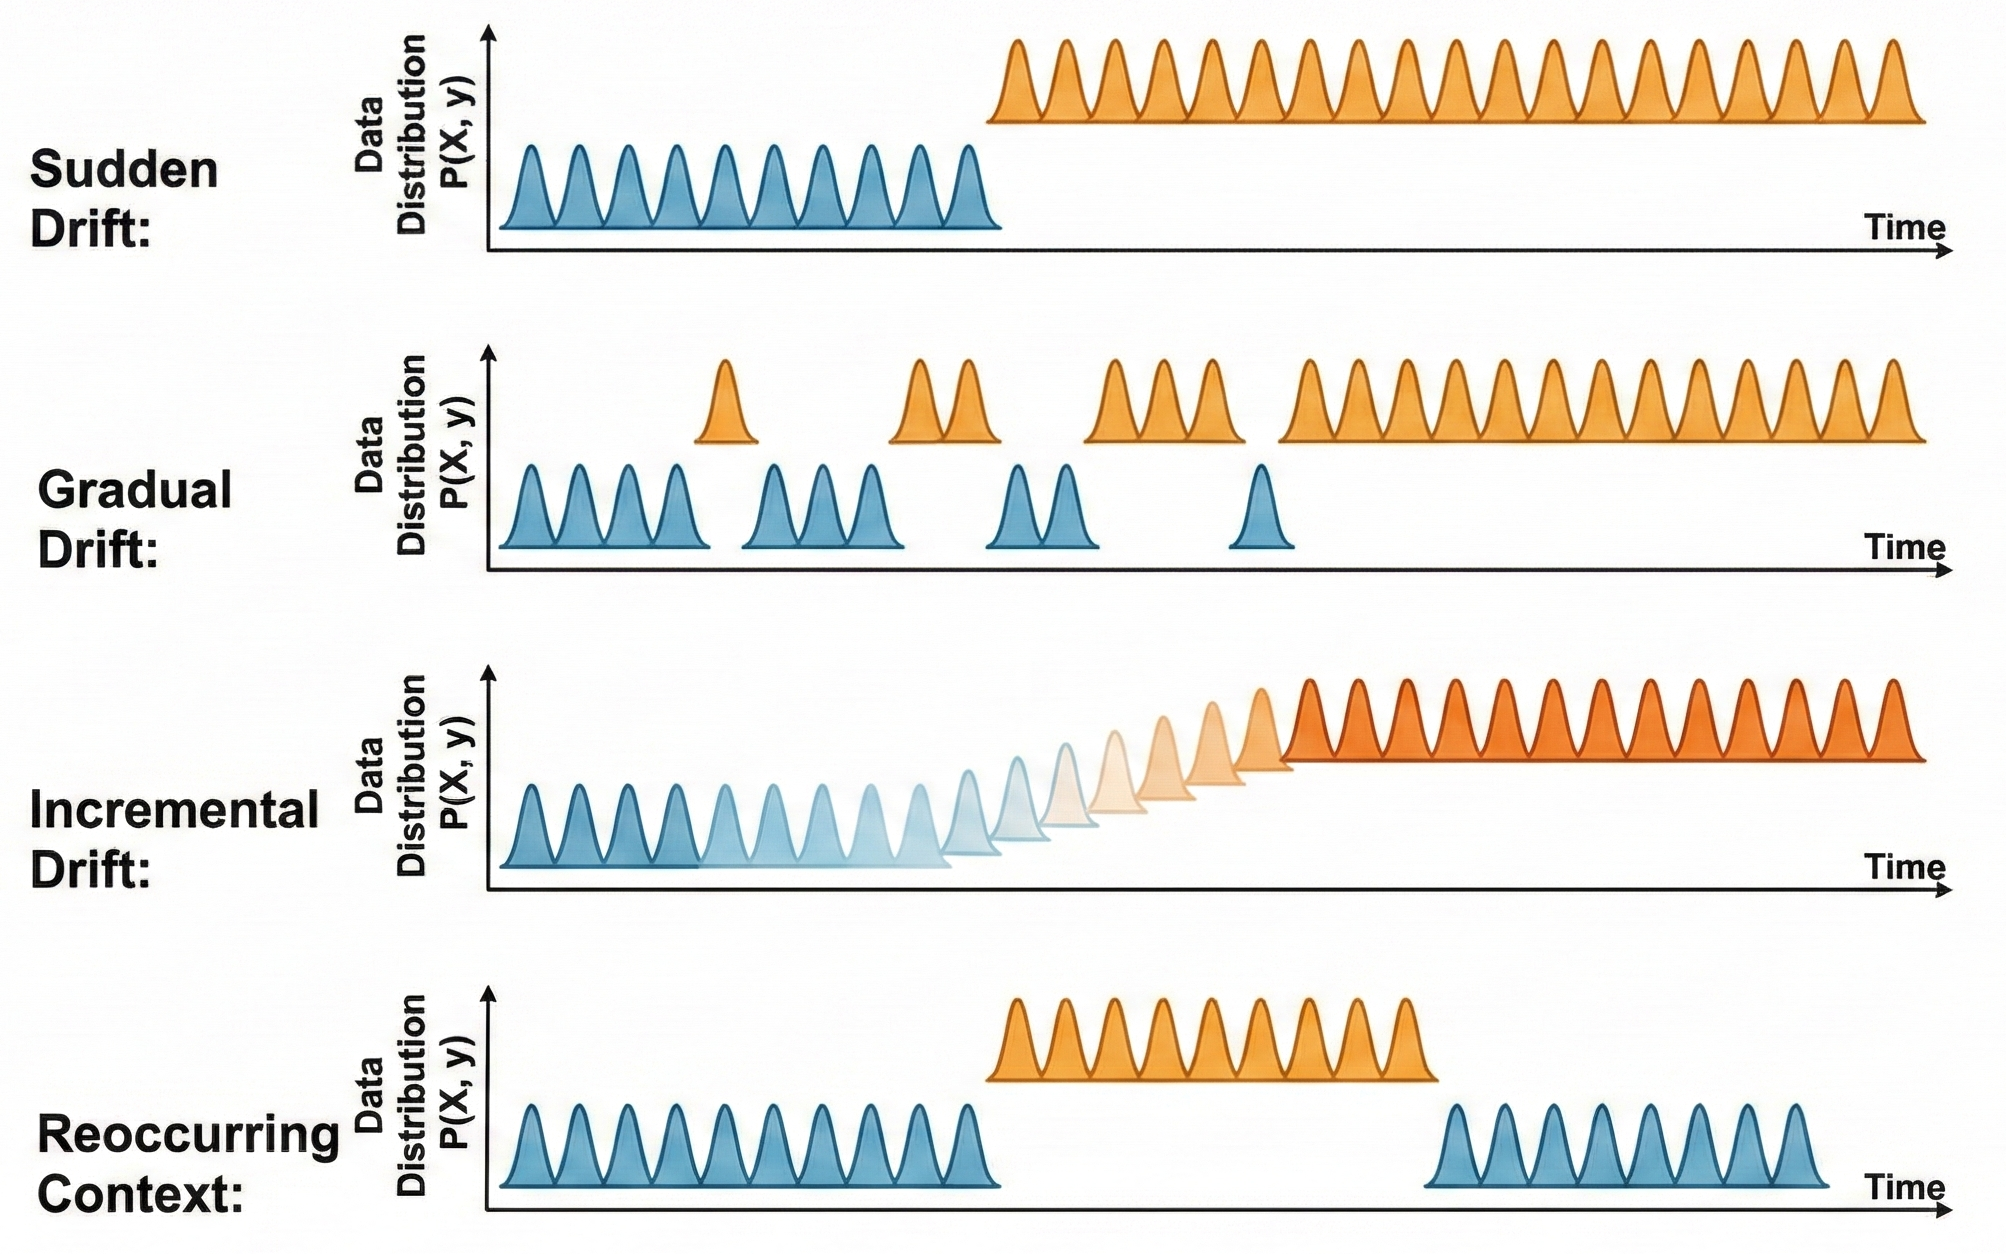
\includegraphics[width=0.75\columnwidth]{images/type_of_drift_detection.png}
    \caption{Types of concept drifts.}
    \label{fig:type_of_drift}
\end{figure}

Over the past two decades, numerous drift detection methods have been developed to address this challenge, including error rate-based approaches such as DDM \cite{Gama2004DDM}, ADWIN \cite{Bifet2007ADWIN}, and ADDM \cite{Mayaki2022ADDM}, distribution-based methods like KSWIN \cite{Raab2020KSWIN}, uncertainty-based methods such as PUDD \cite{Lu2025PUDD}, and meta-learning techniques like Meta-ADD \cite{Yu2021MetaADD}. However, a fundamental challenge remains unresolved in systematically selecting and configuring the most appropriate drift detector for a given data stream.

%The challenge of detector selection is multifaceted. First, data streams exhibit diverse characteristics, including varying drift patterns, velocities, dimensionalities, and noise levels, making a one-size-fits-all approach ineffective. Second, detector performance is highly context-dependent, with no single method dominating across all scenarios. Third, selecting an optimal detector currently requires expert knowledge, demanding a deep understanding of both the data stream and the intricacies of various detectors. Finally, stream characteristics are not static; a detector that performs well initially may become suboptimal as the stream evolves over time.

Automated Machine Learning (AutoML) has revolutionized the field by addressing similar selection challenges in batch learning scenarios \cite{Hutter2019AutoML}. Recent advancements have extended AutoML to streaming data, enabling automatic selection and configuration of classifiers \cite{Celik2023OAML,Verma2024ASML}. However, these systems treat drift detection as a fixed component, requiring manual specification and leaving a critical gap in the automation framework

% To bridge this gap, we introduce \textbf{AutoDD} (Automated Drift Detector), a novel framework that jointly automates the selection and configuration of drift detectors using a cascading bandit approach. The key contributions of this work are:

% \begin{itemize}
% \item \textbf{Cascading Selection Framework:} We propose a two-level hierarchical selection algorithm using LinUCB \cite{Li2010LinUCB} and Thompson Sampling \cite{Agrawal2012Thompson}, which adaptively selects both detectors and their hyperparameter configurations based on online meta-features capturing stream velocity, stationarity, and temporal patterns.

% \item \textbf{Theoretical Analysis:} We formalize detector selection as a contextual bandit problem and provide sublinear regret bounds, guaranteeing convergence to optimal detector selection.

% \item \textbf{Extensive Evaluation:} Through comprehensive experiments on multiple datasets against various baselines, including recent state-of-the-art detectors, we demonstrate that AutoDD consistently outperforms existing approaches while maintaining computational efficiency over learning-based alternatives.
% \end{itemize}

To bridge this gap, we introduce \textbf{AutoDD} (Automated Drift Detector), a novel framework that jointly automates detector selection and configuration using a hierarchical bandit approach. 

\begin{itemize}
\item We propose a two-level hierarchical selection algorithm using LinUCB \cite{Li2010LinUCB} and Thompson Sampling \cite{Agrawal2012Thompson} that adaptively selects detectors and their hyperparameters based on online meta-features.
\item We formalize detector selection with a theoretical analysis provides sublinear regret bounds guaranteeing convergence to optimal selections.
\item Extensive evaluation demonstrates AutoDD outperforms state-of-the-art detectors while maintaining computational efficiency.
\end{itemize}

The rest of this paper is organized as follows. Section~\ref{sec:related} presents the related work. Section~\ref{sec:method} provides the details of our proposed AutoDD framework. Section~\ref{sec:experiments} describes the experimental setup. Section~\ref{sec:results} presents the experimental results and analysis. %Section~\ref{sec:discussion} addresses key design decisions and limitations. 
Finally, Section~\ref{sec:conclusion} concludes the paper.

\section{Related Work}
\label{sec:related}

Drift detection methods can be broadly categorized into three paradigms. \textbf{Error rate-based methods} monitor fluctuations in classifier error rates, triggering alarms when changes are statistically significant. DDM \cite{Gama2004DDM} pioneered the warning-drift framework by monitoring prediction accuracy under binomial distribution assumptions, followed by EDDM \cite{BaenaGarcia2006EDDM} which focuses on distances between errors to detect gradual drift, HDDM \cite{FriasBlanco2015Hoeffding} which applies Hoeffding's inequality with exponentially weighted moving averages, and ADWIN \cite{Bifet2007ADWIN} which maintains adaptive sliding windows that automatically shrink when distribution changes are detected. Page-Hinkley \cite{Page1954Continuous} applies cumulative sum control charts to detect mean shifts in sequential data. Recent advances include MDDM \cite{Pesaranghader2017MDDM}, which uses McDiarmid's inequality for shorter detection delays with tighter concentration bounds, and ADDM \cite{Mayaki2022ADDM}, which models error rates as SETAR time series \cite{Tsay1989TestingAM} to achieve lower false alarm rates. \textbf{Distribution-based methods} compare data distributions across windows by quantifying dissimilarity between new and historical data distributions \cite{Kifer2004ChangeDetection}, including approaches based on information theory \cite{Dasu2006InformationTheoretic}, competence models \cite{Lu2014CompetenceModels}, and the Kolmogorov-Smirnov test (KSWIN) \cite{Raab2020KSWIN} which detects changes in univariate feature distributions. \textbf{Uncertainty and learning-based methods} address limitations of error-rate monitoring: PUDD \cite{Lu2025PUDD} leverages prediction confidence for earlier detection by monitoring changes in prediction uncertainty distributions, while Meta-ADD \cite{Yu2021MetaADD} employs prototypical networks to classify drift types (sudden, gradual, incremental) via meta-learning on diverse drift scenarios.

Recent developments in automated algorithm selection and hyperparameter optimization (CASH) \cite{Hutter2019AutoML} have been extended to streaming scenarios. 
%OAML \cite{Celik2023OAML} uses evolutionary search with drift-triggered reoptimization, while ASML \cite{Verma2024ASML} employs adaptive random directed nearby search with ensemble maintenance to automate classifier selection. 
However, all existing streaming AutoML systems assume a pre-selected drift detector, requiring manual specification and leaving a critical gap in the automation framework. Despite advances in both drift detection and streaming AutoML, drift detector selection remains manual. Our work fills this gap by extending AutoML to automatic drift detector selection and configuration.


\section{Automated Drift Detector}
\label{sec:method}

In this section, we elaborate on Automated Drift Detector (AutoDD). As illustrated in Figure~\ref{fig:framework}, AutoDD employs a closed-loop architecture with the following main steps. First, the system initializes the detector portfolio with standard hyperparameters and sets up the contextual bandit parameters. Then, during online operation, meta-features characterizing stream velocity, stationarity, and temporal patterns are continuously extracted from the incoming data stream. These meta-features serve as context for the LinUCB agent, which selects the most appropriate detector from the portfolio. Subsequently, Thompson Sampling configures the selected detector's hyperparameters for optimal performance. The configured detector monitors the stream and triggers model adaptation upon detecting drift. Finally, performance feedback is computed based on detection outcomes and accuracy changes, which updates both the LinUCB and Thompson Sampling components to refine future selections. This adaptive learning cycle enables AutoDD to continuously improve its detector-stream matching over time.

\begin{figure*}[!t]
    \centering
    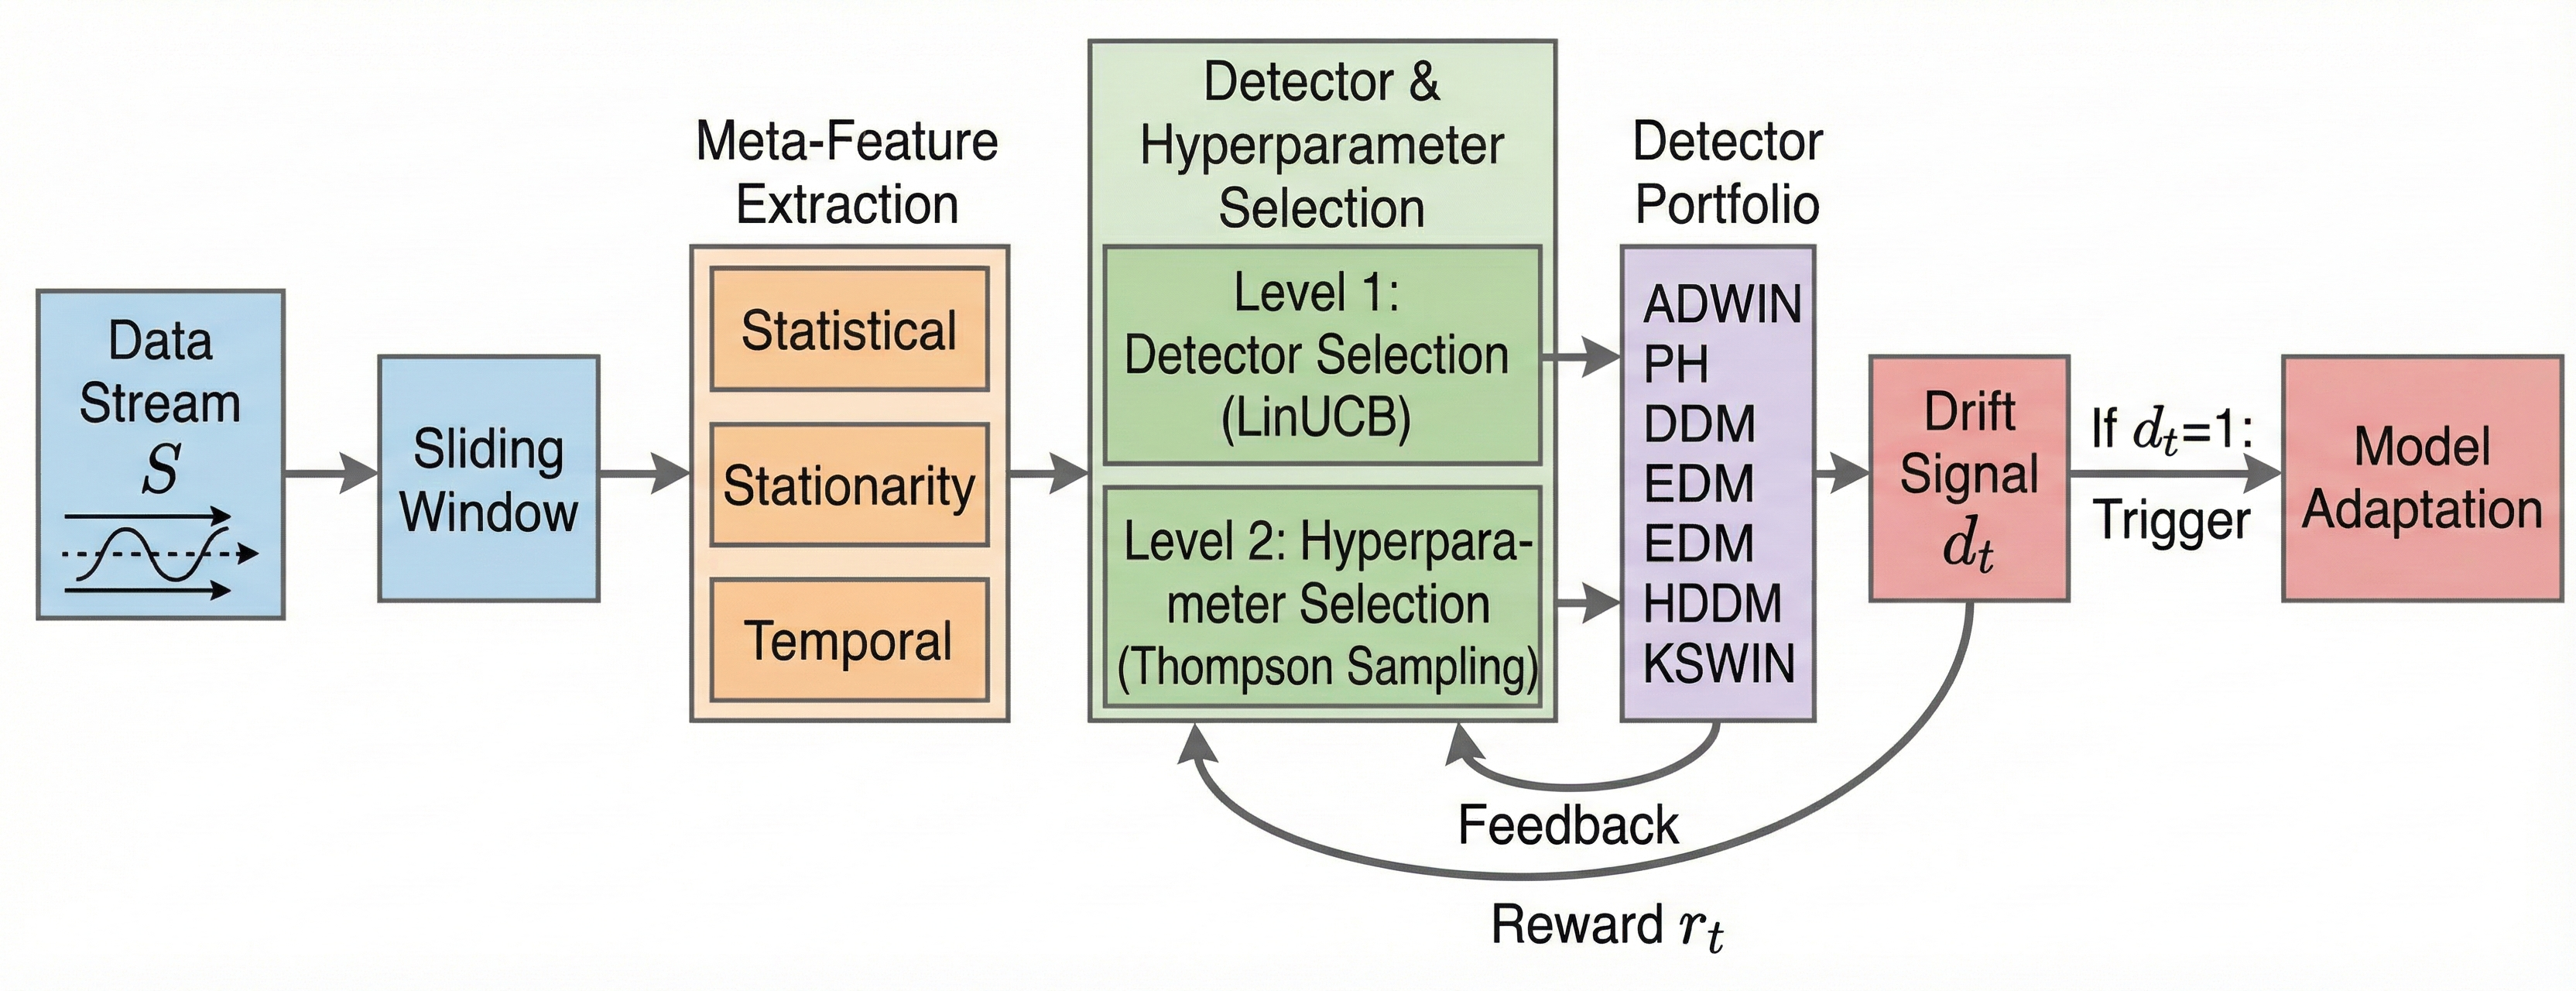
\includegraphics[width=0.75\textwidth]{images/framework_diagram.png}
    \caption{The AutoDD framework consisting of meta-feature extraction, LinUCB-based selection agent, and detector portfolio. The agent adaptively selects detectors based on stream characteristics and updates its policy through performance feedback.}
    \label{fig:framework}
\end{figure*}

\subsection{Algorithm Overview}

AutoDD operates over sliding windows of size $w$. When each window fills with incoming instances, the framework executes a complete selection-detection-update cycle. This cycle begins with extracting stream meta-features.

% \textbf{Meta-Feature Extraction.} We design 15 meta-features organized into three categories, computed efficiently using online statistics. \textit{Statistical meta-features} capture distributional properties: velocity (instance arrival rate), dimensionality (feature space dimension $d$), sparsity (proportion of zero-valued features), noise level (estimated via k-NN entropy with $k=5$), and class imbalance (majority-to-minority class ratio). The velocity is computed as:
% \begin{equation}
% v_t = \frac{n_t}{\Delta t}
% \end{equation}

% \textit{Stationarity meta-features} indicate stream stability: error volatility (standard deviation of error rates), KL divergence (distribution divergence between consecutive windows using histogram-based density estimation with $\sqrt{w}$ adaptive bins), autocorrelation (temporal correlation of error rates), mean shift (average change in feature means), and variance shift (average change in feature variances). The error volatility is:
% \begin{equation}
% \sigma_{err}(t) = \sqrt{\frac{1}{w}\sum_{i=t-w}^{t}(e_i - \bar{e})^2}
% \end{equation}

% \textit{Temporal meta-features} characterize drift behavior: trend (linear regression slope of error rates), periodicity (dominant frequencies via Fourier transform), change frequency (significant changes per unit time), change magnitude (average size of detected shifts), and recurrence score (degree of pattern repetition). All features are normalized to $[0, 1]$ using running min-max statistics, and the context vector $\boldsymbol{\phi}_t \in \mathbb{R}^{15}$ is computed incrementally using Welford's online algorithm and exponential moving averages, ensuring $O(1)$ update complexity per instance.

\textbf{Meta-Feature Extraction:} We design 15 meta-features organized into three categories - Statistical, Stationarity, and Temporal. Table~\ref{tab:metafeatures} summarizes each meta-feature with its mathematical formulation. All features are computed over a sliding window of size $w$ using online statistics and normalized to $[0, 1]$ using running min-max statistics to ensure scale consistency. The context vector $\boldsymbol{\phi}_t \in \mathbb{R}^{15}$ is computed incrementally, ensuring optimum update complexity per instance.

\begin{table}[!ht]
\centering
\caption{Meta-feature portfolio with mathematical formulations}
\label{tab:metafeatures}
\resizebox{\columnwidth}{!}{%
\begin{tabular}{lll}
\toprule
\textbf{Category} & \textbf{Feature} & \textbf{Formula/Description} \\
\midrule
\multirow{5}{*}{Statistical} & Velocity & $v_t = n_t/\Delta t$ \\
& Dimensionality & $d$ \\
& Sparsity & $\frac{1}{wd}\sum_{i=1}^{w}\sum_{j=1}^{d}\mathbb{I}[\mathbf{x}_{i,j}=0]$ \\
& Noise level & $H(\mathbf{X}) \approx -\frac{1}{w}\sum_{i=1}^{w}\log \hat{p}_k(\mathbf{x}_i)$ (k-NN, $k=5$) \\
& Class imbalance & $\max_c |C_c| / \min_c |C_c|$ \\
\midrule
\multirow{5}{*}{Stationarity} & Error volatility & $\sigma_{err}(t) = \sqrt{\frac{1}{w}\sum_{i=t-w}^{t}(e_i - \bar{e})^2}$ \\
& KL divergence & $D_{KL}(P_t \| P_{t-1})$ (histogram, $\sqrt{w}$ bins) \\
& Autocorrelation & $\rho_t = \frac{\text{Cov}(e_t, e_{t-1})}{\sigma_{e_t}\sigma_{e_{t-1}}}$ \\
& Mean shift & $\Delta\mu_t = \frac{1}{d}\sum_{j=1}^{d}|\mu_{t,j} - \mu_{t-1,j}|$ \\
& Variance shift & $\Delta\sigma^2_t = \frac{1}{d}\sum_{j=1}^{d}|\sigma^2_{t,j} - \sigma^2_{t-1,j}|$ \\
\midrule
\multirow{5}{*}{Temporal} & Trend & $\beta = \frac{\text{Cov}(t, e_t)}{\text{Var}(t)}$ \\
& Periodicity & $f_{\text{dom}} = \arg\max_f |\mathcal{F}\{e_t\}(f)|$ \\
& Change frequency & $\frac{1}{\Delta t}\sum_{i=1}^{w}\mathbb{I}[|\Delta e_i| > \tau]$ \\
& Change magnitude & $\frac{1}{|\mathcal{C}_t|}\sum_{i \in \mathcal{C}_t}|\Delta e_i|$ \\
& Recurrence score & $\frac{1}{w^2}\sum_{i,j}\mathbb{I}[d(\mathbf{x}_i, \mathbf{x}_j) < \epsilon]$ \\
\bottomrule
\end{tabular}%
}
\end{table}

\textbf{Detector Portfolio:} AutoDD maintains a diverse portfolio of $K$ drift detectors spanning statistical, error-based, and distribution-based paradigms. Table~\ref{tab:portfolio} summarizes each detector with its hyperparameters, valid ranges, sampling scales, and default values from the literature. For each detector, we maintain $C$ hyperparameter configurations: the first is always the literature default, while the remaining $C-1$ are sampled from the specified ranges using the appropriate scale (logarithmic, linear, or integer).

\begin{table}[!ht]
\centering
\caption{Detector portfolio with hyperparameter configurations}
\label{tab:portfolio}
\resizebox{\columnwidth}{!}{%
\begin{tabular}{llllll}
\toprule
\textbf{Detector} & \textbf{Type} & \textbf{Parameter} & \textbf{Range} & \textbf{Scale} & \textbf{Default} \\
\midrule
\multirow{1}{*}{ADWIN} & Statistical & $\delta$ & [0.0001, 0.1] & log & 0.002 \\
\midrule
\multirow{2}{*}{Page-Hinkley} & \multirow{2}{*}{Statistical} & $\theta$ & [10, 100] & int & 50 \\
& & $\delta$ & [0.001, 0.01] & log & 0.005 \\
\midrule
\multirow{2}{*}{DDM} & \multirow{2}{*}{Error-based} & $w_{thresh}$ & [1.5, 3.0] & linear & 2.0 \\
& & $d_{thresh}$ & [2.0, 4.0] & linear & 3.0 \\
\midrule
\multirow{2}{*}{EDDM} & \multirow{2}{*}{Error-based} & $\alpha$ & [0.90, 0.99] & linear & 0.95 \\
& & $\beta$ & [0.85, 0.95] & linear & 0.90 \\
\midrule
HDDM-A & Error-based & $\delta_d$ & [0.0001, 0.01] & log & 0.001 \\
\midrule
HDDM-W & Error-based & $\lambda$ & [0.01, 0.1] & log & 0.05 \\
\midrule
\multirow{2}{*}{KSWIN} & \multirow{2}{*}{Distribution} & $\alpha$ & [0.001, 0.05] & log & 0.005 \\
& & $w$ & [50, 500] & int & 100 \\
\bottomrule
\end{tabular}%
}
\end{table}

\subsection{Hierarchical Selection Method}

AutoDD uses a two-level hierarchical selection strategy that jointly optimizes detector choice and hyperparameter configuration while maintaining computational efficiency. This approach avoids the combinatorial explosion of $K \times C$ configurations by decomposing the problem into sequential decisions.

\textbf{Level 1 - Detector Selection via LinUCB:} We formulate detector selection as a contextual multi-armed bandit problem where context is $\boldsymbol{\phi}_t$ (meta-features), arms are $K$ detectors, and reward is detection performance. LinUCB \cite{Li2010LinUCB} assumes linear reward:
\begin{equation}
r_{i,t} = \boldsymbol{\phi}_t^\top \boldsymbol{\theta}_i + \epsilon_t
\end{equation}
where $\boldsymbol{\theta}_i \in \mathbb{R}^m$ is the parameter vector for detector $i$. The algorithm selects the detector with highest upper confidence bound:
\begin{equation}
\resizebox{0.9\columnwidth}{!}{$
i_t = \arg\max_{i \in [K]} \left( \boldsymbol{\phi}_t^\top \hat{\boldsymbol{\theta}}_i + \alpha \sqrt{\boldsymbol{\phi}_t^\top \mathbf{A}_i^{-1} \boldsymbol{\phi}_t} \right)
$}
\end{equation}
where $\hat{\boldsymbol{\theta}}_i = \mathbf{A}_i^{-1} \mathbf{b}_i$ is the ridge regression estimate, $\mathbf{A}_i = \lambda\mathbf{I} + \sum_{s:i_s=i} \boldsymbol{\phi}_s \boldsymbol{\phi}_s^\top$ is the regularized design matrix, and $\alpha > 0$ controls exploration-exploitation balance.

\textbf{Level 2 - Hyperparameter Selection via Thompson Sampling:} Given the selected detector $D_{i_t}$, we adaptively configure its hyperparameters using Thompson Sampling \cite{Agrawal2012Thompson}. For each configuration $c$ of detector $i$, we maintain Beta distribution parameters $(\alpha_{i,c}, \beta_{i,c})$ initialized to $(1, 1)$. At each window, we sample:
\begin{equation}
\theta_{i_t,c} \sim \text{Beta}(\alpha_{i_t,c}, \beta_{i_t,c}) \quad \forall c \in [C]
\end{equation}
and select configuration:
\begin{equation}
c_t = \arg\max_c \theta_{i_t,c}
\end{equation}

After observing reward $r_t$, we update:
\begin{align}
\alpha_{i_t,c_t} &\gets \alpha_{i_t,c_t} + \tilde{r}_t \\
\beta_{i_t,c_t} &\gets \beta_{i_t,c_t} + (1 - \tilde{r}_t)
\end{align}
where $\tilde{r}_t = (r_t + 1)/2$ normalizes the reward to $[0,1]$. %This cascading approach provides tractability (only $K$ arms at Level 1), specialization (each detector's hyperparameters tuned independently), and fast adaptation (Thompson Sampling quickly identifies effective configurations).

\subsection{Evaluation and Adaptation}

Evaluating detector performance without ground truth drift labels is challenging. Following standard practice, we use model accuracy drop as a proxy metric. The reward at time $t$ is:
\begin{equation}
r_t = \begin{cases}
0.5 + \min(\Delta a \cdot 2, 0.5) & d=1, \Delta a > \tau \\
-0.3 & d=1, \Delta a \leq \tau \\
-0.5 - \min(\Delta a, 0.5) & d=0, \Delta a > \tau \\
0.1 & d=0, \Delta a \leq \tau
\end{cases}
\end{equation}
where $d \in \{0,1\}$ indicates drift detection, $\Delta a = acc_{t-w} - acc_t$ is the accuracy drop between windows, and $\tau = 0.05$ is the significance threshold. The reward function penalizes both false positives and false negatives while rewarding correct drift detections and stable periods.

Upon drift detection, the model undergoes complete reset. Let $\mathcal{M}_t$ denote the classifier state at time $t$. When drift is detected ($d_t = 1$), we perform:
\begin{equation}
\mathcal{M}_t \gets \mathcal{M}_0
\end{equation}
where $\mathcal{M}_0$ represents the initial untrained state. The classifier then resumes incremental learning from subsequent instances:
\begin{equation}
\mathcal{M}_{t+s} \gets \text{Update}(\mathcal{M}_{t+s-1}, (\mathbf{x}_{t+s}, y_{t+s})) \quad \forall s > 0
\end{equation}

The complete procedure is formalized in Algorithm~\ref{alg:autodd}.

\begin{algorithm}[t]
\caption{AutoDD Algorithm}
\label{alg:autodd}
\textbf{Input:} Stream $\mathcal{S}$, Portfolio $\mathcal{D}$, HP configs $\mathcal{C}$, Window $w$\\
\textbf{Parameter:} Exploration $\alpha$, Configs per detector $C$\\
\textbf{Output:} Drift signals $\{d_t\}_{t=1}^\infty$
\begin{algorithmic}[1]
\STATE Initialize $\mathbf{A}_i \gets \mathbf{I}_m$, $\mathbf{b}_i \gets \mathbf{0}$ for all $i \in [K]$
\STATE Initialize $\alpha_{i,c} \gets 1$, $\beta_{i,c} \gets 1$ for all $i \in [K], c \in [C]$
\STATE Initialize sliding window $W \gets \emptyset$
\FOR{each instance $(\mathbf{x}_t, y_t) \in \mathcal{S}$}
    \STATE $W \gets W \cup \{(\mathbf{x}_t, y_t)\}$
    \IF{$|W| = w$}
        \STATE Extract meta-features $\boldsymbol{\phi}_t \gets \textsc{Extract}(W)$
        %\STATE \textit{// Level 1: Detector Selection (LinUCB)}
        \FOR{$i = 1$ to $K$}
            \STATE $\text{UCB}_i \gets \boldsymbol{\phi}_t^\top \mathbf{A}_i^{-1} \mathbf{b}_i + \alpha \sqrt{\boldsymbol{\phi}_t^\top \mathbf{A}_i^{-1} \boldsymbol{\phi}_t}$
        \ENDFOR
        \STATE Select detector $i_t \gets \arg\max_i \text{UCB}_i$
        %\STATE \textit{// Level 2: Hyperparameter Selection (Thompson Sampling)}
        \FOR{$c = 1$ to $C$}
            \STATE Sample $\theta_c \sim \text{Beta}(\alpha_{i_t,c}, \beta_{i_t,c})$
        \ENDFOR
        \STATE Select config $c_t \gets \arg\max_c \theta_c$
        \STATE $d_t \gets D_{i_t}(\mathcal{C}_{i_t,c_t}).\textsc{Detect}(W)$
        \IF{$d_t = 1$}
            \STATE $\mathcal{M}_t \gets \mathcal{M}_0$ %\textit{// Reset classifier to initial state}
        \ENDIF
        \STATE Compute reward $r_t$ using Eq. (7)
        %\STATE \textit{// Update Level 1 (LinUCB)}
        \STATE $\mathbf{A}_{i_t} \gets \mathbf{A}_{i_t} + \boldsymbol{\phi}_t \boldsymbol{\phi}_t^\top$; $\mathbf{b}_{i_t} \gets \mathbf{b}_{i_t} + r_t \boldsymbol{\phi}_t$
        %\STATE \textit{// Update Level 2 (Thompson Sampling)}
        \STATE $\tilde{r}_t \gets (r_t + 1)/2$
        \STATE $\alpha_{i_t,c_t} \gets \alpha_{i_t,c_t} + \tilde{r}_t$; $\beta_{i_t,c_t} \gets \beta_{i_t,c_t} + (1-\tilde{r}_t)$
        \STATE $W \gets \emptyset$
    \ENDIF
\ENDFOR
\end{algorithmic}
\end{algorithm}

\subsection{Computational Complexity}
AutoDD has per-window complexity of $O(wd + Km^2)$, where $w$ is window size, $d$ is feature dimensionality, $K$ is the number of detectors, and $m$ is meta-feature count. The dominant costs are meta-feature extraction ($O(wd)$) and LinUCB matrix operations ($O(Km^2)$). Space complexity is $O(Km^2 + wd)$ for storing $K$ covariance matrices of size $m \times m$ and the sliding window buffer. With $K=7$, $m=15$, and $w=100$, these remain constant regardless of stream length, ensuring scalability to unbounded streams.

% \subsection{Theoretical Analysis}

% We formalize AutoDD's optimization objective and provide regret guarantees for the hierarchical bandit approach.

% \textbf{Problem Formulation.} A data stream $\mathcal{S} = \{(\mathbf{x}_t, y_t)\}_{t=1}^{\infty}$ exhibits concept drift when distributions change:
% \begin{equation}
% \exists t, t' : P_t(\mathbf{X}, Y) \neq P_{t'}(\mathbf{X}, Y)
% \end{equation}

% Given detector portfolio $\mathcal{D} = \{D_1, \ldots, D_K\}$ where each $D_i$ has configuration space $\Lambda_i$, AutoDD solves the streaming CASH problem \cite{Hutter2019AutoML}:
% \begin{equation}
% \resizebox{0.95\columnwidth}{!}{$
% (D^*_t, \lambda^*_t) = \arg\max_{D_i \in \mathcal{D}, \lambda \in \Lambda_i} \mathbb{E}[\mathcal{M}(D_i(\lambda), \mathcal{S}_t) \mid \boldsymbol{\phi}_t]
% $}
% \end{equation}
% where $\boldsymbol{\phi}_t$ is the stream context. The hierarchical approach decomposes this into two sequential decisions: detector selection (Level 1) and hyperparameter configuration (Level 2).

% \textbf{Assumptions.} We make three standard assumptions:
% \begin{itemize}
% \item \textbf{(A1) Bounded features:} $\|\boldsymbol{\phi}_t\|_2 \leq L$ for all $t$, satisfied by $[0,1]$ normalization.
% \item \textbf{(A2) Linear reward:} For each detector $i$, there exists $\boldsymbol{\theta}_i^* \in \mathbb{R}^m$ with $\|\boldsymbol{\theta}_i^*\|_2 \leq S$ such that $\mathbb{E}[r_{i,t} \mid \boldsymbol{\phi}_t] = \boldsymbol{\phi}_t^\top \boldsymbol{\theta}_i^*$.
% \item \textbf{(A3) Sub-Gaussian noise:} Reward noise is $\sigma$-sub-Gaussian, holding with $\sigma = 1$ for bounded rewards.
% \end{itemize}

% \textbf{Theorem 1 (Level 1 Regret).} Under assumptions A1--A3, with exploration parameter $\alpha = \sigma\sqrt{m \log(KT/\delta)} + S$, LinUCB detector selection achieves with probability at least $1 - \delta$:
% \begin{equation}
% \resizebox{0.95\columnwidth}{!}{$
% R_1(T) = \sum_{t=1}^{T} \left( \max_{i} \boldsymbol{\phi}_t^\top \boldsymbol{\theta}_i^* - \boldsymbol{\phi}_t^\top \boldsymbol{\theta}_{i_t}^* \right) = O(\sqrt{mT \log T})
% $}
% \end{equation}

% \textit{Proof sketch.} Follows standard LinUCB analysis \cite{Li2010LinUCB,Abbasi2011Improved} via confidence ellipsoids from self-normalized martingale bounds, instantaneous regret bounds from UCB selection, and summation using the elliptical potential lemma. Full proof appears in supplementary material.

% \textbf{Theorem 2 (Level 2 Regret).} For Thompson Sampling on $C$ configurations per detector, with $N_i(T)$ selections of detector $i$, the cumulative regret satisfies:
% \begin{equation}
% R_2(T) = \sum_{i=1}^{K} O(\sqrt{C \cdot N_i(T) \log N_i(T)})
% \end{equation}

% \textit{Proof sketch.} Applies the Bayesian regret bound for Beta-Bernoulli Thompson Sampling \cite{Agrawal2012Thompson}, treating each detector's configuration selection as an independent bandit conditioned on detector selection.

% \textbf{Corollary (Combined Regret).} The total regret combines both levels:
% \begin{equation}
% R(T) = R_1(T) + R_2(T) = O(\sqrt{mT \log T} + \sqrt{CKT \log T})
% \end{equation}

% This sublinear regret guarantees convergence to optimal detector-configuration pairs:
% \begin{equation}
% \lim_{T \to \infty} \frac{R(T)}{T} = 0
% \end{equation}

% \textbf{Sample Complexity.} To achieve average regret $\epsilon$, AutoDD requires:
% \begin{equation}
% T = O\left(\frac{(m + CK) \log(K/\delta)}{\epsilon^2}\right)
% \end{equation}

\subsection{Theoretical Analysis}

We formalize AutoDD's optimization objective and provide regret guarantees for the hierarchical bandit approach.

\textbf{Problem Formulation.} A data stream $\mathcal{S} = \{(\mathbf{x}_t, y_t)\}_{t=1}^{\infty}$ exhibits concept drift when distributions change:
\begin{equation}
\exists t, t' : P_t(\mathbf{X}, Y) \neq P_{t'}(\mathbf{X}, Y)
\end{equation}

Given detector portfolio $\mathcal{D} = \{D_1, \ldots, D_K\}$ where each $D_i$ has configuration space $\Lambda_i$, AutoDD solves the streaming CASH problem \cite{Hutter2019AutoML}:
\begin{equation}
\resizebox{0.95\columnwidth}{!}{$
(D^*_t, \lambda^*_t) = \arg\max_{D_i \in \mathcal{D}, \lambda \in \Lambda_i} \mathbb{E}[\mathcal{M}(D_i(\lambda), \mathcal{S}_t) \mid \boldsymbol{\phi}_t]
$}
\end{equation}
where $\boldsymbol{\phi}_t$ is the stream context. The hierarchical approach decomposes this into two sequential decisions: detector selection (Level 1) and hyperparameter configuration (Level 2).

\textbf{Assumptions.} We make three standard assumptions from the contextual bandit literature \cite{Abbasi2011Improved,Lattimore2020Bandit}:
\begin{itemize}
\item \textbf{(A1) Bounded features:} $\|\boldsymbol{\phi}_t\|_2 \leq L$ for all $t$, satisfied by $[0,1]$ normalization with $L=\sqrt{m}$.
\item \textbf{(A2) Linear reward:} For each detector $i$, there exists $\boldsymbol{\theta}_i^* \in \mathbb{R}^m$ with $\|\boldsymbol{\theta}_i^*\|_2 \leq S$ such that $\mathbb{E}[r_{i,t} \mid \boldsymbol{\phi}_t] = \boldsymbol{\phi}_t^\top \boldsymbol{\theta}_i^*$.
\item \textbf{(A3) Sub-Gaussian noise:} Reward noise is $\sigma$-sub-Gaussian, holding with $\sigma = 1$ for bounded rewards in $[-1,1]$.
\end{itemize}

\textbf{Theorem 1 (Level 1 Regret).} Under assumptions A1--A3, with exploration parameter $\alpha = \sigma\sqrt{m \log(KT/\delta)} + S$, LinUCB detector selection achieves with probability at least $1 - \delta$:
\begin{equation}
\resizebox{0.95\columnwidth}{!}{$
R_1(T) = \sum_{t=1}^{T} \left( \max_{i} \boldsymbol{\phi}_t^\top \boldsymbol{\theta}_i^* - \boldsymbol{\phi}_t^\top \boldsymbol{\theta}_{i_t}^* \right) = O(\sqrt{mT \log T})
$}
\end{equation}

\textit{Proof.} The proof follows directly from Theorem 2 of \cite{Abbasi2011Improved}. By the self-normalized martingale inequality (Theorem 1, \cite{Abbasi2011Improved}), the true parameter $\boldsymbol{\theta}_i^*$ lies within the confidence ellipsoid $\mathcal{C}_{i,t} = \{\boldsymbol{\theta}: \|\boldsymbol{\theta} - \hat{\boldsymbol{\theta}}_i\|_{\mathbf{A}_i} \leq \alpha\}$ with probability $1-\delta$. Under this event, UCB selection ensures $\boldsymbol{\phi}_t^\top \boldsymbol{\theta}_{i_t}^* \geq \max_i \boldsymbol{\phi}_t^\top \boldsymbol{\theta}_i^* - 2\alpha\|\boldsymbol{\phi}_t\|_{\mathbf{A}_{i_t}^{-1}}$. Summing and applying the elliptical potential lemma \cite{Dani2008Stochastic} yields $\sum_{t=1}^T \|\boldsymbol{\phi}_t\|_{\mathbf{A}_{i_t}^{-1}} \leq \sqrt{2mT\log(1+TL^2/m)}$, giving the stated bound. \hfill $\square$

\textbf{Theorem 2 (Level 2 Regret).} For Thompson Sampling on $C$ configurations per detector, with $N_i(T)$ selections of detector $i$, the cumulative regret satisfies:
\begin{equation}
R_2(T) = \sum_{i=1}^{K} O(\sqrt{C \cdot N_i(T) \log N_i(T)})
\end{equation}

\textit{Proof.} Conditioned on detector $i$ being selected, hyperparameter selection reduces to a $C$-armed bandit. We normalize bounded rewards $r_t \in [-1,1]$ to $\tilde{r}_t = (r_t+1)/2 \in [0,1]$ and treat them as pseudo-Bernoulli outcomes for Beta-Bernoulli Thompson Sampling. By Theorem 1 of \cite{Agrawal2013Further}, Thompson Sampling with Beta priors achieves expected regret $O(\sqrt{CN_i(T)\log N_i(T)})$ over $N_i(T)$ rounds for bounded rewards. Since detector selections partition the time horizon ($\sum_i N_i(T) = T$), summing across detectors yields the stated bound. \hfill $\square$

\textbf{Corollary (Combined Regret).} The total regret of the hierarchical system is:
\begin{equation}
R(T) = R_1(T) + R_2(T) = O(\sqrt{mT \log T} + \sqrt{CKT \log T})
\end{equation}

\textit{Proof.} By Cauchy-Schwarz, $\sum_i \sqrt{N_i(T)} \leq \sqrt{K \sum_i N_i(T)} = \sqrt{KT}$. Thus $R_2(T) = O(\sqrt{CKT\log T})$, and adding $R_1(T)$ gives the result. \hfill $\square$

This sublinear regret guarantees convergence to optimal detector-configuration pairs:
\begin{equation}
\lim_{T \to \infty} \frac{R(T)}{T} = 0
\end{equation}

\textbf{Sample Complexity.} To achieve average regret $\epsilon$, AutoDD requires $T = O\left(\frac{(m + CK) \log(K/\delta)}{\epsilon^2}\right)$ samples, following from inverting the regret bound.



\section{Experiments}
\label{sec:experiments}

% \subsection{Experimental Setup}

% \textbf{Datasets.} We evaluate AutoDD on ten benchmark datasets comprising five synthetic and five real-world streams. Table~\ref{tab:datasets} summarizes their characteristics. Synthetic datasets are generated using River's stream generators with predefined drift points, while real-world datasets are standard benchmarks from the MOA framework \cite{Bifet2010MOA}.

% \begin{table}[!ht]
% \centering
% \caption{Dataset characteristics (Multiple* = Sudden, Gradual, Incremental, and Normal drift types)}
% \label{tab:datasets}
% \begin{tabular}{llrrll}
% \toprule
% \textbf{Dataset} & \textbf{Type} & \textbf{Instances} & \textbf{Features} & \textbf{Drift Type} \\
% \midrule
% SEA & Synthetic & 500,000 & 3 & Multiple* \\
% HYP & Synthetic & 500,000 & 10 & Multiple* \\
% AGR & Synthetic & 100,000 & 9 & Multiple* \\
% RBF & Synthetic & 200,000 & 10 & Multiple* \\
% RTG & Synthetic & 100,000 & 30 & Multiple* \\
% \midrule
% Elec & Real-world & 45,312 & 8 & Unknown \\
% Weather & Real-world & 18,159 & 8 & Unknown \\
% Spam & Real-world & 4,601 & 57 & Unknown \\
% Airlines & Real-world & 539,383 & 7 & Unknown \\
% Poker & Real-world & 829,201 & 10 & Unknown \\
% \bottomrule
% \end{tabular}
% \end{table}

% \textbf{Baselines.} We compare AutoDD against twelve baselines: (1) GaussianNB without drift detection (*), (2-8) seven individual detectors from AutoDD's portfolio (ADWIN, DDM, EDDM, HDDM-A, HDDM-W, Page-Hinkley, KSWIN), (9-11) three recent state-of-the-art detectors---MDDM \cite{Pesaranghader2017MDDM} using McDiarmid's inequality, ADDM \cite{Mayaki2022ADDM} using autoregressive modeling, and PUDD \cite{Lu2025PUDD} using prediction uncertainty---and (12) Meta-ADD \cite{Yu2021MetaADD}, a meta-learning approach using prototypical networks. All detectors use recommended hyperparameter settings from the literature.

% \textbf{Metrics.} We measure: (1) \textit{Prequential accuracy}---percentage of correct predictions using test-then-train evaluation, (2) \textit{F1-score}---harmonic mean of drift detection precision and recall (synthetic only), (3) \textit{Drift count}---number of detected drifts (real-world only), and (4) \textit{Computational cost}---runtime per instance and memory usage.

% \textbf{F1 Evaluation Protocol.} For synthetic datasets with known drift points, we match detected drifts to ground truth using a tolerance window of $\delta=100$ instances, following standard practice \cite{Bifet2007ADWIN}. A detection is a \textit{true positive} if it falls within $\pm\delta$ of an unmatched true drift; each true drift can match at most one detection (first-match greedy). Multiple alarms near the same drift contribute to false positives. Zero F1 scores in Table~\ref{tab:synthetic} occur when a detector fails to trigger any alarm within the tolerance window of any true drift---common for detectors with high thresholds (e.g., ADWIN on HYP) or those designed for different drift types than present in the stream.

% \textbf{Configuration.} AutoDD uses all 15 meta-features with window size $w=100$, exploration parameter $\alpha=1.0$, and $C=5$ hyperparameter configurations per detector (1 default + 4 sampled). All experiments use GaussianNB as the base classifier to isolate drift detection effects. Results are averaged over 10 runs. Implementation uses Python with River \cite{Montiel2021River} on a MacBook Pro with Apple M2 Pro and 16GB RAM.

% All experiments are fully reproducible; the implementation and datasets are publicly available.\footnote{Dataset and code available at: \url{https://anonymous.4open.science/r/AutoDD-BCCF}}

%\subsection{Experimental Setup}

We evaluate AutoDD on ten benchmark datasets comprising five synthetic and five real-world streams (Table~\ref{tab:datasets}). Synthetic datasets are generated using River's~\cite{montiel2021river} stream generators with predefined drift points exhibiting multiple drift types (sudden, gradual, incremental, and normal), while real-world datasets are standard benchmarks from the MOA framework \cite{Bifet2010MOA} with unknown drift patterns. To demonstrate robustness, we evaluate all methods using two base classifiers: GaussianNB and Hoeffding Adaptive Tree (HAT)~\cite{domingos2000mining}. We compare AutoDD against twelve baselines: a no-detector baseline, seven individual detectors from AutoDD's portfolio (ADWIN, DDM, EDDM, HDDM-A, HDDM-W, Page-Hinkley, KSWIN), and four recent state-of-the-art methods including MDDM \cite{Pesaranghader2017MDDM}, ADDM \cite{Mayaki2022ADDM}, PUDD \cite{Lu2025PUDD}, and Meta-ADD \cite{Yu2021MetaADD}. All detectors use recommended hyperparameter settings from the literature.

\begin{table}[!ht]
\centering
\caption{Dataset characteristics (Multiple* = Sudden, Gradual, Incremental, and Normal drift types)}
\label{tab:datasets}
\resizebox{\columnwidth}{!}{%
\begin{tabular}{llrrll}
\toprule
\textbf{Dataset} & \textbf{Type} & \textbf{Instances} & \textbf{Features} & \textbf{Drift Type} \\
\midrule
SEA & Synthetic & 500,000 & 3 & Multiple* \\
HYP & Synthetic & 500,000 & 10 & Multiple* \\
AGR & Synthetic & 100,000 & 9 & Multiple* \\
RBF & Synthetic & 200,000 & 10 & Multiple* \\
RTG & Synthetic & 100,000 & 30 & Multiple* \\
\midrule
Elec & Real-world & 45,312 & 8 & Unknown \\
Weather & Real-world & 18,159 & 8 & Unknown \\
Spam & Real-world & 4,601 & 57 & Unknown \\
Airlines & Real-world & 539,383 & 7 & Unknown \\
Poker & Real-world & 829,201 & 10 & Unknown \\
\bottomrule
\end{tabular}%
}
\end{table}

We measure prequential accuracy as the percentage of correct predictions using test-then-train evaluation. For synthetic datasets with known drift points, we report F1-score computed by matching detected drifts to ground truth using a tolerance window of $\delta=100$ instances following standard practice \cite{Bifet2007ADWIN}. For real-world datasets, we report the number of detected drifts (DN). AutoDD uses all 15 meta-features with window size $w=100$, exploration parameter $\alpha=1.0$, and $C=5$ hyperparameter configurations per detector. Results are averaged over 10 runs. Implementation uses Python with River~\cite{montiel2021river} on a MacBook Pro with Apple M2 Pro and 16GB RAM.\footnote{Code and datasets: \url{https://anonymous.4open.science/r/AutoDD-BCCF}}

\section{Results}
\label{sec:results}

We conduct comprehensive evaluation comparing AutoDD with classical detectors and state-of-the-art methods across both base classifiers.

\textbf{Synthetic Datasets:} Table~\ref{tab:synthetic} presents results on synthetic benchmarks with known drift points. AutoDD consistently achieves the highest mean accuracy across both base classifiers, demonstrating robust performance regardless of the underlying learning paradigm. With GaussianNB, AutoDD attains 81.9\% mean accuracy, while with HAT it reaches 84.0\%, outperforming all state-of-the-art detectors in both settings. Meta-ADD ranks as the second-best method, achieving 80.9\% with GaussianNB and 81.4\% with HAT. AutoDD demonstrates particular strength on datasets with abrupt drift patterns, where its ability to rapidly switch between detectors provides substantial benefits. On the SEA dataset, AutoDD achieves 93.1\% accuracy with GaussianNB and 96.7\% with HAT, significantly outperforming all baselines. Similar improvements are observed on the AGR dataset with 78.5\% and 82.4\% accuracy respectively. Meta-ADD performs competitively on gradual drift scenarios due to its learned drift-type representations. Notably, fixed detectors exhibit inconsistent performance across different drift types, with HDDM-W achieving strong results on some datasets but underperforming on others, highlighting the fundamental need for adaptive detector selection.

% \begin{table*}[!ht]
% \centering
% \caption{Results on synthetic datasets. Best results in \textbf{bold}.}
% \label{tab:synthetic_old}
% \resizebox{0.75\textwidth}{!}{%
% \begin{tabular}{l|cc|cc|cc|cc|cc|cc}
% \toprule
% & \multicolumn{2}{c|}{\textbf{SEA}} & \multicolumn{2}{c|}{\textbf{HYP}} & \multicolumn{2}{c|}{\textbf{AGR}} & \multicolumn{2}{c|}{\textbf{RBF}} & \multicolumn{2}{c|}{\textbf{RTG}} & \multicolumn{2}{c}{\textbf{Mean}} \\
% & Acc & F1 & Acc & F1 & Acc & F1 & Acc & F1 & Acc & F1 & Acc & F1 \\
% \midrule
% No Detector & 83.8 & 0.40 & 76.4 & 0.34 & 78.8 & 0.41 & 50.4 & 0.09 & 58.2 & 0.10 & 69.5 & 0.27 \\
% ADWIN & 84.0 & 0.61 & 81.9 & 0.00 & 71.5 & 0.51 & 69.6 & 0.00 & 64.5 & 0.00 & 74.3 & 0.22 \\
% DDM & 83.8 & 0.00 & 86.1 & 0.63 & 71.6 & 0.49 & 71.3 & 0.64 & 64.4 & 0.00 & 75.4 & 0.35 \\
% EDDM & 84.3 & 0.40 & 85.7 & 0.63 & 65.3 & 0.24 & 67.7 & 0.38 & 65.0 & 0.40 & 73.6 & 0.41 \\
% HDDM-A & 84.6 & 0.69 & 81.5 & 0.00 & 72.2 & 0.63 & 69.7 & 0.00 & 64.4 & 0.00 & 74.5 & 0.26 \\
% HDDM-W & 84.4 & 0.66 & 86.6 & 0.71 & 73.1 & 0.67 & 70.1 & 0.51 & 65.8 & 0.56 & 76.0 & 0.62 \\
% Page-Hinkley & 84.7 & 0.70 & 81.5 & 0.00 & 71.5 & 0.49 & 69.4 & 0.00 & 64.5 & 0.00 & 74.3 & 0.24 \\
% KSWIN & 83.7 & 0.35 & 85.7 & 0.65 & 71.5 & 0.50 & 70.0 & 0.61 & 65.2 & 0.39 & 75.2 & 0.50 \\
% \midrule
% MDDM & 86.7 & 0.65 & 87.2 & 0.68 & 72.3 & 0.71 & 69.8 & 0.56 & 66.1 & 0.56 & 76.4 & 0.63 \\
% ADDM & 87.7 & 0.83 & 88.7 & 0.73 & 73.6 & 0.67 & 70.9 & 0.62 & 67.6 & 0.71 & 77.7 & 0.71 \\
% PUDD & 86.2 & 0.81 & 89.5 & 0.84 & 73.7 & 0.72 & 73.4 & 0.72 & 67.8 & 0.71 & 78.1 & 0.76 \\
% Meta-ADD & 88.9 & 0.87 & 90.8 & \textbf{0.91} & 74.1 & 0.79 & \textbf{78.0} & 0.70 & \textbf{72.9} & 0.76 & 80.9 & 0.81 \\
% \textbf{AutoDD} & \textbf{93.1} & \textbf{0.90} & \textbf{94.6} & 0.91 & \textbf{78.5} & \textbf{0.84} & 74.3 & \textbf{0.81} & 69.2 & \textbf{0.84} & \textbf{81.9} & \textbf{0.86} \\
% \bottomrule
% \end{tabular}%
% }
% \end{table*}

\begin{table*}[!ht]
\centering
\caption{Results on synthetic datasets with both base classifiers. \textbf{Bold}: best, \underline{Underline}: second-best.}
\label{tab:synthetic}
\resizebox{\textwidth}{!}{%
\begin{tabular}{l|cc|cc|cc|cc|cc|cc||cc|cc|cc|cc|cc|cc}
\toprule
& \multicolumn{12}{c||}{\textbf{GaussianNB (GNB)}} & \multicolumn{12}{c}{\textbf{Hoeffding Adaptive Tree (HAT)}} \\
\cmidrule{2-25}
& \multicolumn{2}{c|}{\textbf{SEA}} & \multicolumn{2}{c|}{\textbf{HYP}} & \multicolumn{2}{c|}{\textbf{AGR}} & \multicolumn{2}{c|}{\textbf{RBF}} & \multicolumn{2}{c|}{\textbf{RTG}} & \multicolumn{2}{c||}{\textbf{Mean}} & \multicolumn{2}{c|}{\textbf{SEA}} & \multicolumn{2}{c|}{\textbf{HYP}} & \multicolumn{2}{c|}{\textbf{AGR}} & \multicolumn{2}{c|}{\textbf{RBF}} & \multicolumn{2}{c|}{\textbf{RTG}} & \multicolumn{2}{c}{\textbf{Mean}} \\
& Acc & F1 & Acc & F1 & Acc & F1 & Acc & F1 & Acc & F1 & Acc & F1 & Acc & F1 & Acc & F1 & Acc & F1 & Acc & F1 & Acc & F1 & Acc & F1 \\
\midrule
No Detector & 83.8 & 0.40 & 76.4 & 0.34 & 78.8 & 0.41 & 50.4 & 0.09 & 58.2 & 0.10 & 69.5 & 0.27 & 86.2 & 0.42 & 79.1 & 0.36 & 81.3 & 0.43 & 53.1 & 0.11 & 60.8 & 0.12 & 72.1 & 0.29 \\
ADWIN & 84.0 & 0.61 & 81.9 & 0.00 & 71.5 & 0.51 & 69.6 & 0.00 & 64.5 & 0.00 & 74.3 & 0.22 & 88.1 & 0.64 & 85.5 & 0.06 & 74.6 & 0.55 & 73.3 & 0.07 & 68.3 & 0.11 & 77.9 & 0.29 \\
DDM & 83.8 & 0.00 & 86.1 & 0.63 & 71.6 & 0.49 & 71.3 & 0.64 & 64.4 & 0.00 & 75.4 & 0.35 & 88.0 & 0.10 & 89.0 & 0.67 & 74.7 & 0.52 & 74.6 & 0.69 & 68.1 & 0.13 & 78.9 & 0.42 \\
EDDM & 84.3 & 0.40 & 85.7 & 0.63 & 65.3 & 0.24 & 67.7 & 0.38 & 65.0 & 0.40 & 73.6 & 0.41 & 88.0 & 0.46 & 88.6 & 0.68 & 69.2 & 0.29 & 71.8 & 0.42 & 68.8 & 0.47 & 77.3 & 0.46 \\
HDDM-A & 84.6 & 0.69 & 81.5 & 0.00 & 72.2 & 0.63 & 69.7 & 0.00 & 64.4 & 0.00 & 74.5 & 0.26 & 88.3 & 0.64 & 86.8 & 0.06 & 75.1 & 0.63 & 73.8 & 0.07 & 69.1 & 0.11 & 78.6 & 0.30 \\
HDDM-W & 84.4 & 0.66 & 86.6 & 0.71 & 73.1 & 0.67 & 70.1 & 0.51 & 65.8 & 0.56 & 76.0 & 0.62 & 88.4 & 0.65 & 89.5 & 0.72 & 75.9 & 0.67 & 73.9 & 0.53 & 69.7 & 0.58 & 79.5 & 0.63 \\
Page-Hinkley & 84.7 & 0.70 & 81.5 & 0.00 & 71.5 & 0.49 & 69.4 & 0.00 & 64.5 & 0.00 & 74.3 & 0.24 & 88.2 & 0.65 & 86.0 & 0.06 & 74.8 & 0.52 & 73.5 & 0.07 & 68.5 & 0.11 & 78.2 & 0.28 \\
KSWIN & 83.7 & 0.35 & 85.7 & 0.65 & 71.5 & 0.50 & 70.0 & 0.61 & 65.2 & 0.39 & 75.2 & 0.50 & 88.0 & 0.42 & 88.3 & 0.66 & 74.5 & 0.53 & 73.7 & 0.63 & 68.9 & 0.43 & 78.7 & 0.53 \\
\midrule
MDDM & 86.7 & 0.65 & 87.2 & 0.68 & 72.3 & 0.71 & 69.8 & 0.56 & 66.1 & 0.56 & 76.4 & 0.63 & 89.1 & 0.67 & 90.3 & 0.75 & 75.5 & 0.75 & 73.8 & 0.60 & 69.8 & 0.61 & 78.4 & 0.68 \\
ADDM & 87.7 & 0.83 & 88.7 & 0.73 & 73.6 & 0.67 & 70.9 & 0.62 & 67.6 & 0.71 & 77.7 & 0.71 & 89.8 & 0.86 & 91.9 & 0.77 & 76.6 & 0.72 & 75.0 & 0.69 & 71.3 & 0.77 & 79.3 & 0.76 \\
PUDD & 86.2 & 0.81 & 89.5 & \underline{0.84} & 73.7 & 0.72 & \underline{73.4} & \underline{0.72} & 67.8 & 0.71 & 78.1 & 0.76 & 89.8 & 0.83 & \underline{92.6} & 0.83 & \underline{77.1} & 0.76 & \underline{76.4} & \underline{0.74} & \underline{71.9} & 0.74 & 79.7 & 0.78 \\
Meta-ADD & \underline{88.9} & \underline{0.87} & \underline{90.8} & \textbf{0.91} & \underline{74.1} & \underline{0.79} & \textbf{78.0} & 0.70 & \textbf{72.9} & \underline{0.76} & \underline{80.9} & \underline{0.81} & \underline{90.9} & \underline{0.91} & 92.5 & \underline{0.92} & \underline{77.1} & \underline{0.81} & \textbf{84.8} & \underline{0.74} & \textbf{80.4} & \underline{0.79} & \underline{81.4} & \underline{0.83} \\
\textbf{AutoDD} & \textbf{93.1} & \textbf{0.90} & \textbf{94.6} & \textbf{0.91} & \textbf{78.5} & \textbf{0.84} & 74.3 & \textbf{0.81} & \underline{69.2} & \textbf{0.84} & \textbf{81.9} & \textbf{0.86} & \textbf{96.7} & \textbf{0.93} & \textbf{98.4} & \textbf{0.93} & \textbf{82.4} & \textbf{0.90} & 75.8 & \textbf{0.84} & 70.9 & \textbf{0.88} & \textbf{84.0} & \textbf{0.87} \\
\bottomrule
\end{tabular}%
}
\end{table*}

\textbf{Real-world Datasets:} Table~\ref{tab:realworld} presents results on real-world benchmarks where drift patterns are unknown and potentially more complex than synthetic scenarios. AutoDD demonstrates strong generalization, achieving the highest mean accuracy with both base classifiers. With GaussianNB, AutoDD attains 79.1\% mean accuracy, improving to 83.1\% with HAT, consistently outperforming all state-of-the-art detectors. ADDM emerges as the second-best performer with 75.1\% accuracy using GaussianNB and 77.8\% with HAT. AutoDD's improvements are consistent across all five real-world datasets, demonstrating that its adaptive selection mechanism generalizes well to diverse application domains. On the Electricity dataset, AutoDD achieves 89.6\% with GaussianNB and 93.8\% with HAT. On Weather, it reaches 80.0\% and 85.1\% respectively, while on Spam it attains near-perfect accuracy of 97.9\% and 99.0\%. Importantly, AutoDD maintains well-balanced drift detection behavior, avoiding both over-detection and under-detection patterns that plague fixed detectors. On the Airlines dataset, AutoDD detects 118 drifts, compared to HDDM-W's excessive 269 detections and ADWIN's insufficient 76 detections, demonstrating appropriate sensitivity calibration.

% \begin{table*}[!ht]
% \centering
% \caption{Results on real-world datasets. DN = number of detected drifts. Best results in \textbf{bold}.}
% \label{tab:realworld_old}
% \resizebox{0.75\textwidth}{!}{%
% \begin{tabular}{l|cc|cc|cc|cc|cc|cc}
% \toprule
% & \multicolumn{2}{c|}{\textbf{Elec}} & \multicolumn{2}{c|}{\textbf{Weather}} & \multicolumn{2}{c|}{\textbf{Spam}} & \multicolumn{2}{c|}{\textbf{Airlines}} & \multicolumn{2}{c|}{\textbf{Poker}} & \multicolumn{2}{c}{\textbf{Mean}} \\
% & Acc & DN & Acc & DN & Acc & DN & Acc & DN & Acc & DN & Acc & DN \\
% \midrule
% No Detector & 73.2 & 2 & 68.9 & 2 & 77.2 & 1 & 59.3 & 2 & 54.6 & 2 & 66.6 & 1.8 \\
% ADWIN & 79.2 & 22 & 69.3 & 7 & 92.1 & 2 & 62.5 & 76 & 54.3 & 3 & 71.5 & 22.0 \\
% DDM & 82.3 & 22 & 70.6 & 5 & 91.8 & 2 & 61.8 & 20 & 54.2 & 3 & 72.1 & 10.4 \\
% EDDM & 82.4 & 22 & 73.8 & 9 & 92.9 & 2 & 61.3 & 182 & 53.6 & 4 & 72.8 & 43.8 \\
% HDDM-A & 82.7 & 22 & 72.2 & 9 & 92.5 & 2 & 62.6 & 114 & 54.6 & 6 & 72.9 & 30.6 \\
% HDDM-W & 81.9 & 22 & 72.6 & 9 & 91.9 & 1 & 61.0 & 269 & 52.3 & 394 & 72.0 & 139.0 \\
% Page-Hinkley & 78.0 & 16 & 69.4 & 6 & 91.8 & 1 & 62.8 & 64 & 54.3 & 17 & 71.3 & 20.8 \\
% KSWIN & 81.1 & 22 & 68.0 & 9 & 92.6 & 2 & 61.6 & 269 & 53.7 & 266 & 71.4 & 113.6 \\
% \midrule
% MDDM & 83.9 & 22 & 74.8 & 9 & 92.8 & 2 & 62.2 & 110 & 56.1 & 190 & 74.0 & 66.6 \\
% ADDM & 84.8 & 22 & 76.3 & 9 & 93.9 & 2 & 63.9 & 74 & 56.5 & 177 & 75.1 & 56.8 \\
% PUDD & 84.4 & 22 & 75.4 & 9 & 93.2 & 2 & 64.0 & 117 & 56.2 & 81 & 74.6 & 46.2 \\
% Meta-ADD & 85.4 & 22 & 74.9 & 9 & 94.5 & 2 & 63.8 & 139 & 55.5 & 182 & 74.8 & 70.8 \\
% \textbf{AutoDD} & \textbf{89.6} & 22 & \textbf{80.0} & 9 & \textbf{97.9} & 2 & \textbf{68.2} & 118 & \textbf{59.7} & 188 & \textbf{79.1} & 67.8 \\
% \bottomrule
% \end{tabular}%
% }
% \end{table*}

\begin{table*}[!ht]
\centering
\caption{Results on real-world datasets with both base classifiers. DN = detected drifts. \textbf{Bold}: best, \underline{Underline}: second-best.}
\label{tab:realworld}
\resizebox{\textwidth}{!}{%
\begin{tabular}{l|cc|cc|cc|cc|cc|cc||cc|cc|cc|cc|cc|cc}
\toprule
& \multicolumn{12}{c||}{\textbf{GaussianNB (GNB)}} & \multicolumn{12}{c}{\textbf{Hoeffding Adaptive Tree (HAT)}} \\
\cmidrule{2-25}
& \multicolumn{2}{c|}{\textbf{Elec}} & \multicolumn{2}{c|}{\textbf{Weather}} & \multicolumn{2}{c|}{\textbf{Spam}} & \multicolumn{2}{c|}{\textbf{Airlines}} & \multicolumn{2}{c|}{\textbf{Poker}} & \multicolumn{2}{c||}{\textbf{Mean}} & \multicolumn{2}{c|}{\textbf{Elec}} & \multicolumn{2}{c|}{\textbf{Weather}} & \multicolumn{2}{c|}{\textbf{Spam}} & \multicolumn{2}{c|}{\textbf{Airlines}} & \multicolumn{2}{c|}{\textbf{Poker}} & \multicolumn{2}{c}{\textbf{Mean}} \\
& Acc & DN & Acc & DN & Acc & DN & Acc & DN & Acc & DN & Acc & DN & Acc & DN & Acc & DN & Acc & DN & Acc & DN & Acc & DN & Acc & DN \\
\midrule
No Detector & 73.2 & 0 & 68.9 & 0 & 77.2 & 0 & 59.3 & 0 & 54.6 & 0 & 66.6 & 0 & 76.5 & 0 & 71.4 & 0 & 80.1 & 0 & 62.1 & 0 & 56.9 & 0 & 69.4 & 0 \\
ADWIN & 79.2 & 22 & 69.3 & 7 & 92.1 & 2 & 62.5 & 76 & 54.3 & 3 & 71.5 & 22.0 & 82.4 & 22 & 73.1 & 9 & 94.6 & 2 & 66.3 & 76 & 57.7 & 3 & 74.8 & 22.4 \\
DDM & 82.3 & 22 & 70.6 & 5 & 91.8 & 2 & 61.8 & 20 & 54.2 & 3 & 72.1 & 10.4 & 85.5 & 22 & 73.5 & 7 & 93.9 & 2 & 65.2 & 20 & 58.0 & 3 & 75.2 & 10.8 \\
EDDM & 82.4 & 22 & 73.8 & 9 & 92.9 & 2 & 61.3 & 182 & 53.6 & 4 & 72.8 & 43.8 & 85.2 & 22 & 77.1 & 9 & 94.8 & 2 & 64.6 & 182 & 57.8 & 4 & 75.9 & 43.8 \\
HDDM-A & 82.7 & 22 & 72.2 & 9 & 92.5 & 2 & 62.6 & 114 & 54.6 & 6 & 72.9 & 30.6 & 86.3 & 22 & 75.8 & 9 & 94.7 & 2 & 66.1 & 114 & 58.5 & 6 & 76.3 & 30.6 \\
HDDM-W & 81.9 & 22 & 72.6 & 9 & 91.9 & 1 & 61.0 & 269 & 52.3 & 394 & 71.9 & 139.0 & 85.1 & 22 & 76.0 & 9 & 94.5 & 1 & 64.9 & 269 & 56.8 & 404 & 75.5 & 141.0 \\
Page-Hinkley & 78.0 & 16 & 69.4 & 6 & 91.8 & 1 & 62.8 & 64 & 54.3 & 17 & 71.3 & 20.8 & 81.7 & 16 & 72.8 & 6 & 94.2 & 1 & 66.5 & 64 & 57.5 & 17 & 74.5 & 20.8 \\
KSWIN & 81.1 & 22 & 68.0 & 9 & 92.6 & 2 & 61.6 & 269 & 53.7 & 266 & 71.4 & 113.6 & 84.3 & 22 & 71.2 & 9 & 94.9 & 2 & 65.4 & 269 & 57.0 & 266 & 74.6 & 113.6 \\
\midrule
MDDM & 83.9 & 22 & 74.8 & 9 & 92.8 & 2 & 62.2 & 110 & 56.1 & 190 & 74.0 & 66.6 & 86.5 & 22 & 78.0 & 9 & 94.6 & 2 & 66.0 & 110 & \underline{60.0} & 190 & 77.0 & 66.6 \\
ADDM & 84.8 & 22 & \underline{76.3} & 9 & 93.9 & 2 & 63.9 & 74 & \underline{56.5} & 177 & \underline{75.1} & 56.8 & 87.3 & 22 & \underline{79.2} & 9 & 95.8 & 2 & 66.9 & 74 & 59.6 & 177 & \underline{77.8} & 56.8 \\
PUDD & 84.4 & 22 & 75.4 & 9 & 93.2 & 2 & \underline{64.0} & 117 & 56.2 & 81 & 74.6 & 46.2 & 87.5 & 22 & 78.6 & 9 & 95.6 & 2 & \underline{67.7} & 117 & 59.7 & 81 & \underline{77.8} & 46.2 \\
Meta-ADD & \underline{85.4} & 22 & 74.9 & 9 & \underline{94.5} & 2 & 63.8 & 139 & 55.5 & 182 & 74.8 & 70.8 & \underline{87.9} & 22 & 78.2 & 9 & \underline{95.9} & 2 & 66.5 & 139 & 59.6 & 182 & 77.6 & 70.8 \\
\textbf{AutoDD} & \textbf{89.6} & 22 & \textbf{80.0} & 9 & \textbf{97.9} & 2 & \textbf{68.2} & 118 & \textbf{59.7} & 188 & \textbf{79.1} & 67.8 & \textbf{93.8} & 22 & \textbf{85.1} & 9 & \textbf{99.0} & 2 & \textbf{72.6} & 118 & \textbf{65.1} & 188 & \textbf{83.1} & 67.8 \\
\bottomrule
\end{tabular}%
}
\end{table*}

\begin{figure*}[!ht]
    \centering
    \begin{subfigure}[b]{0.24\textwidth}
        \centering
        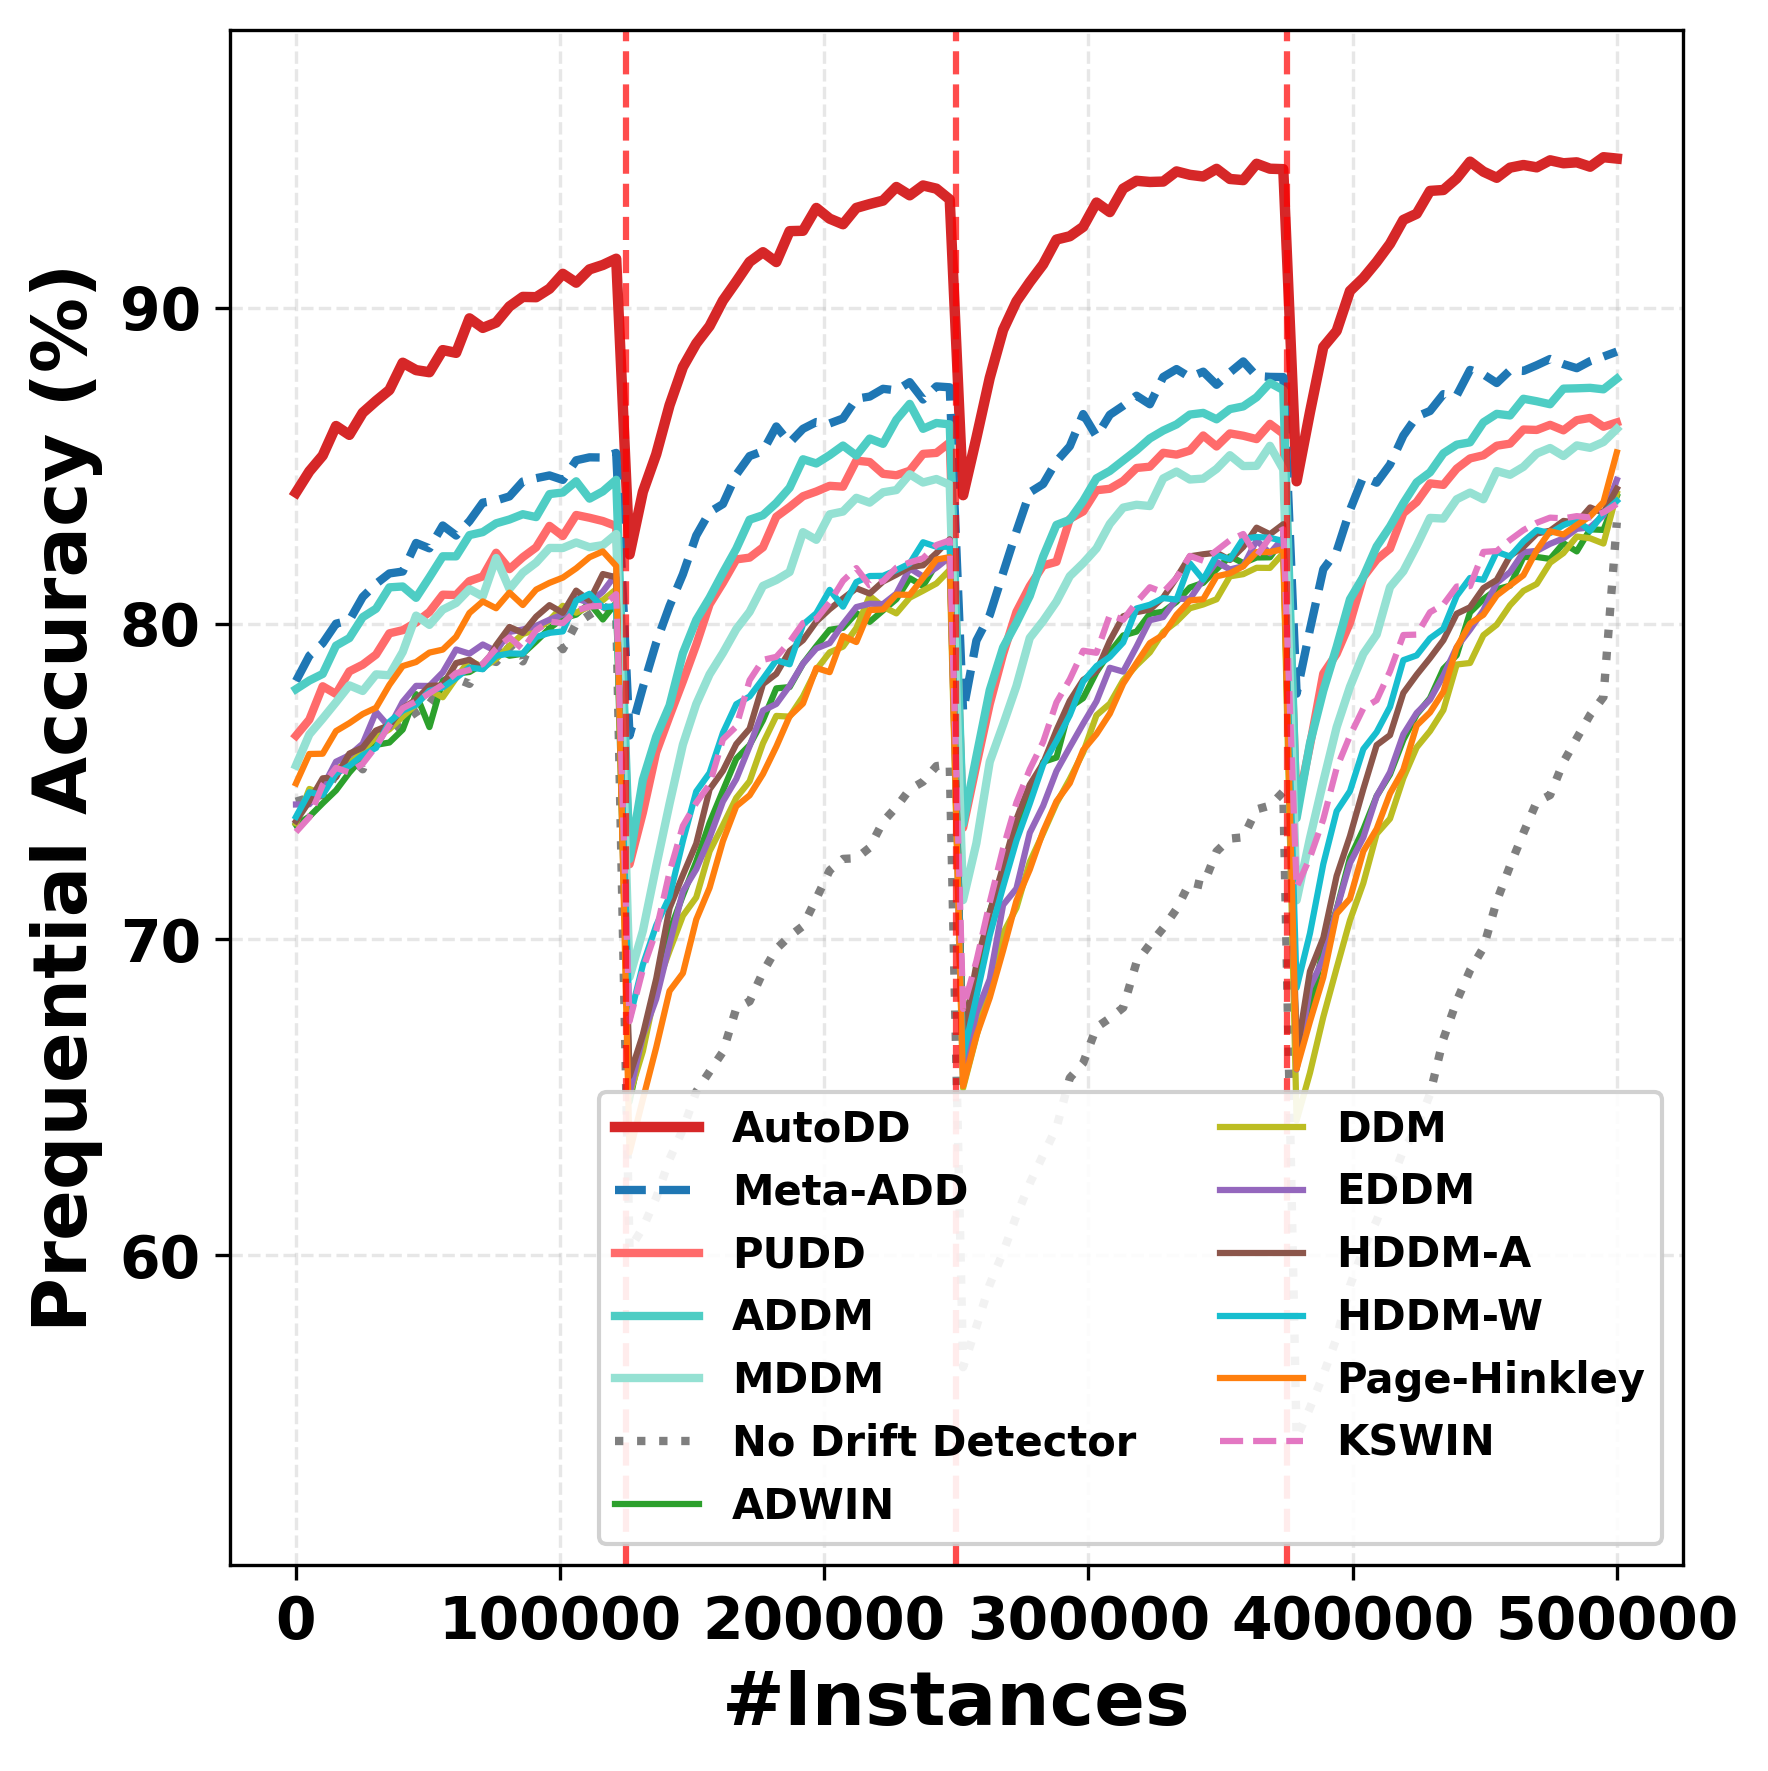
\includegraphics[width=\textwidth]{images/prequential_sea_gaussiannb.png}
        \caption{SEA (GNB)}
    \end{subfigure}
    \hfill
    \begin{subfigure}[b]{0.24\textwidth}
        \centering
        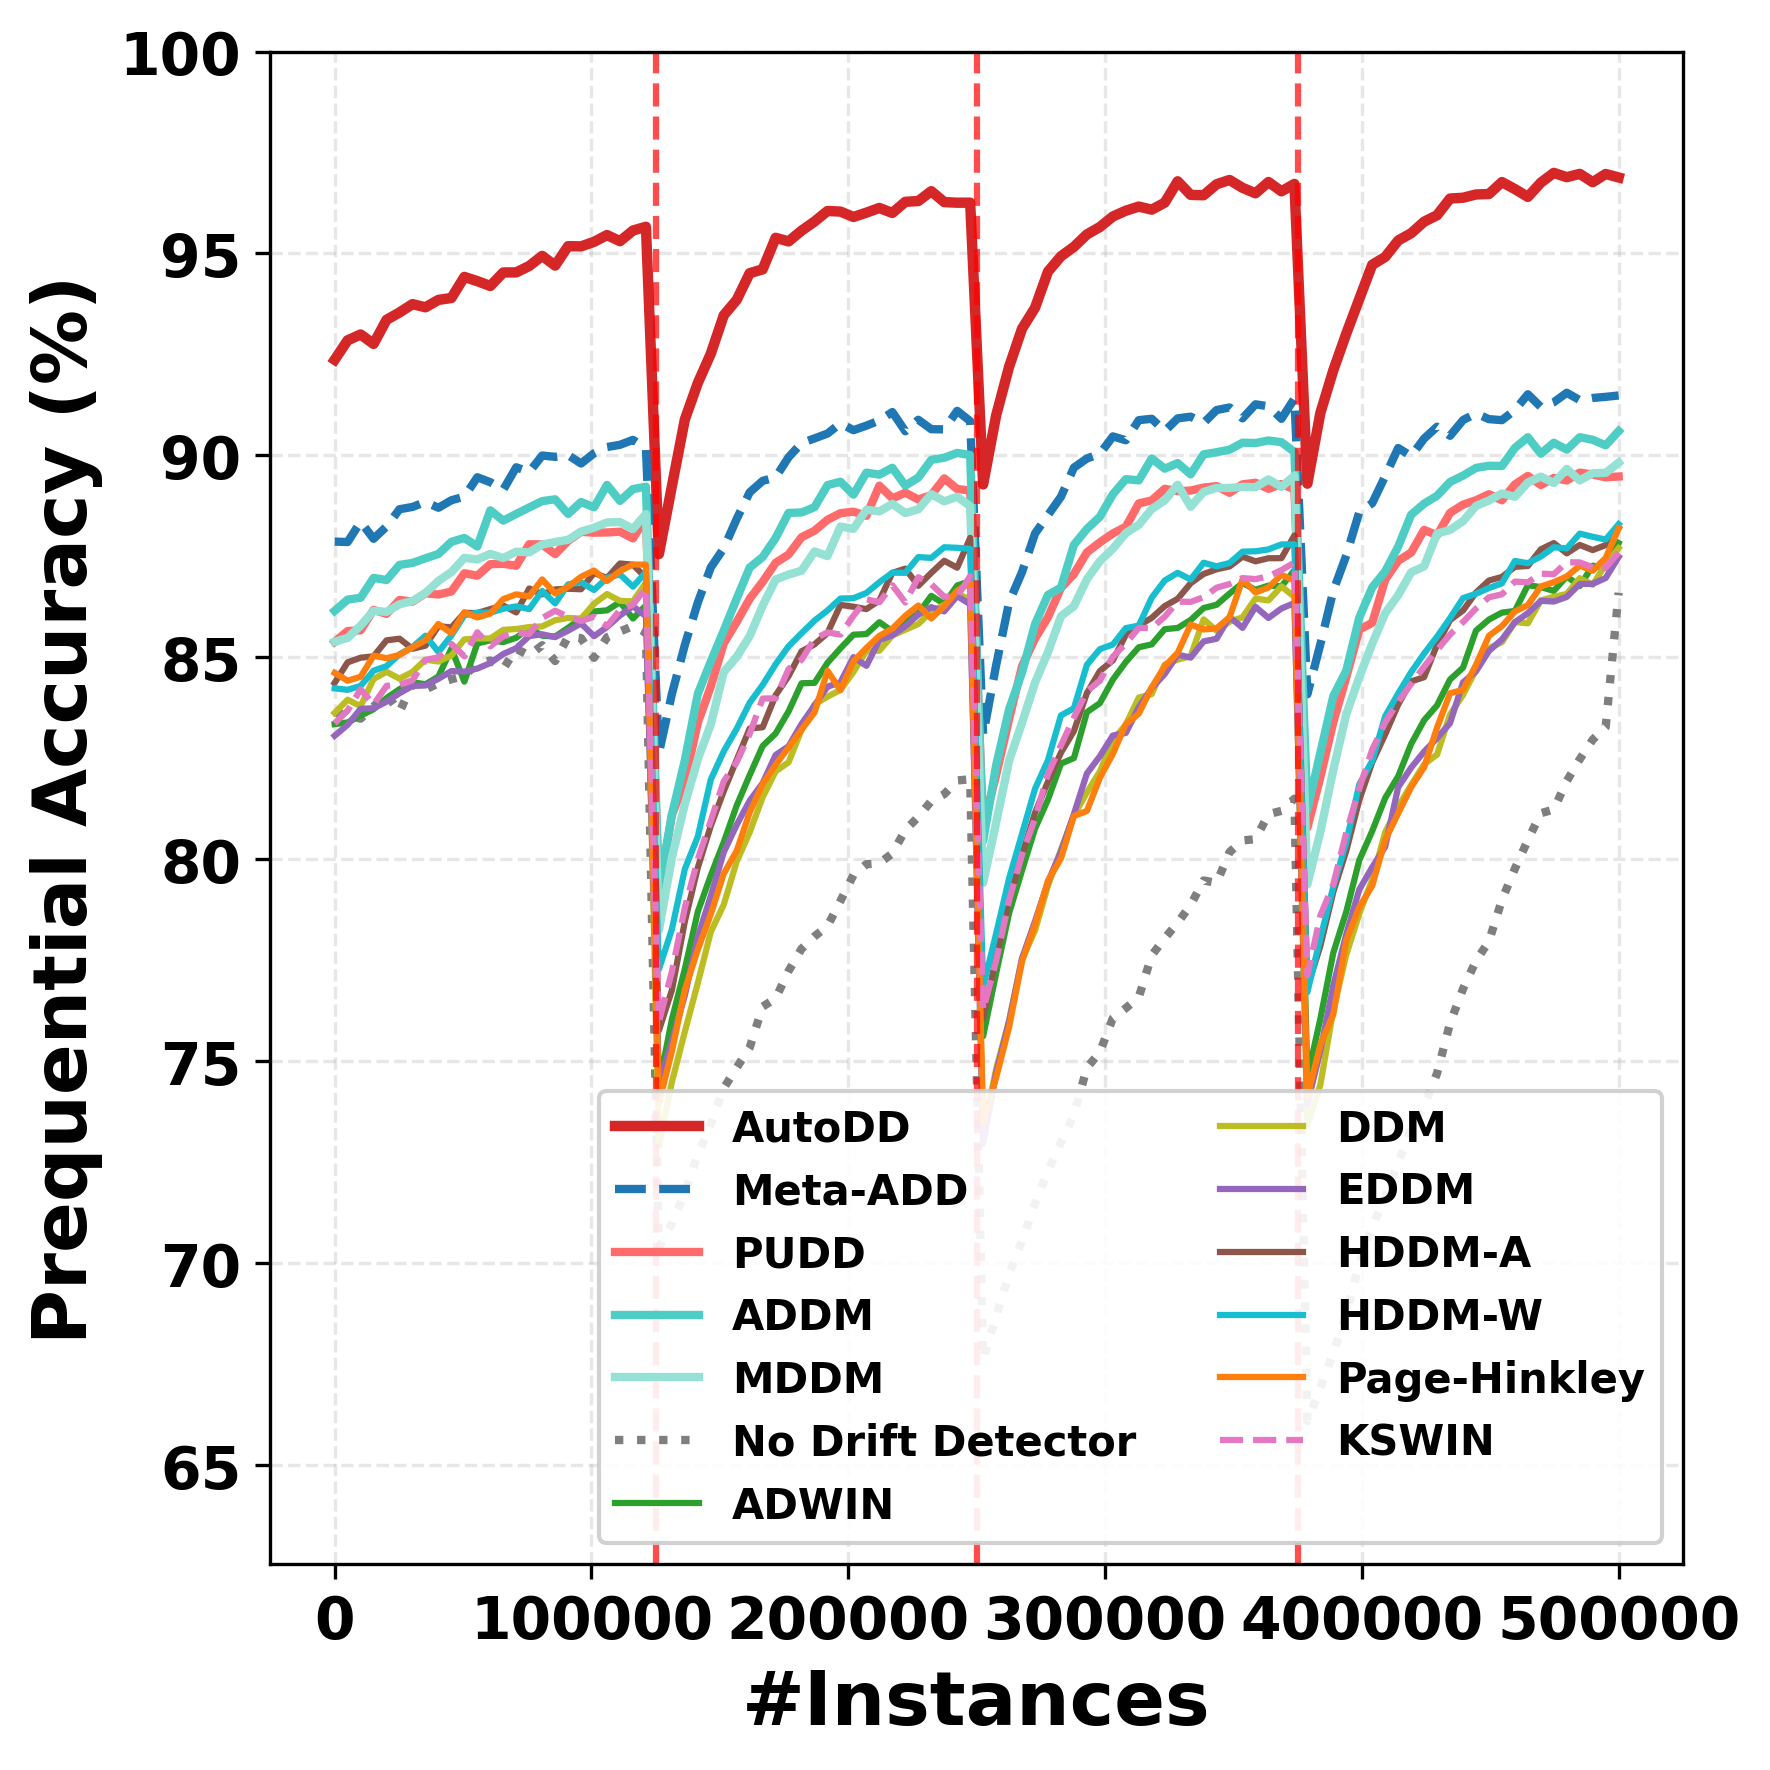
\includegraphics[width=\textwidth]{images/prequential_sea_hat.png}
        \caption{SEA (HAT)}
    \end{subfigure}
    \hfill
    \begin{subfigure}[b]{0.24\textwidth}
        \centering
        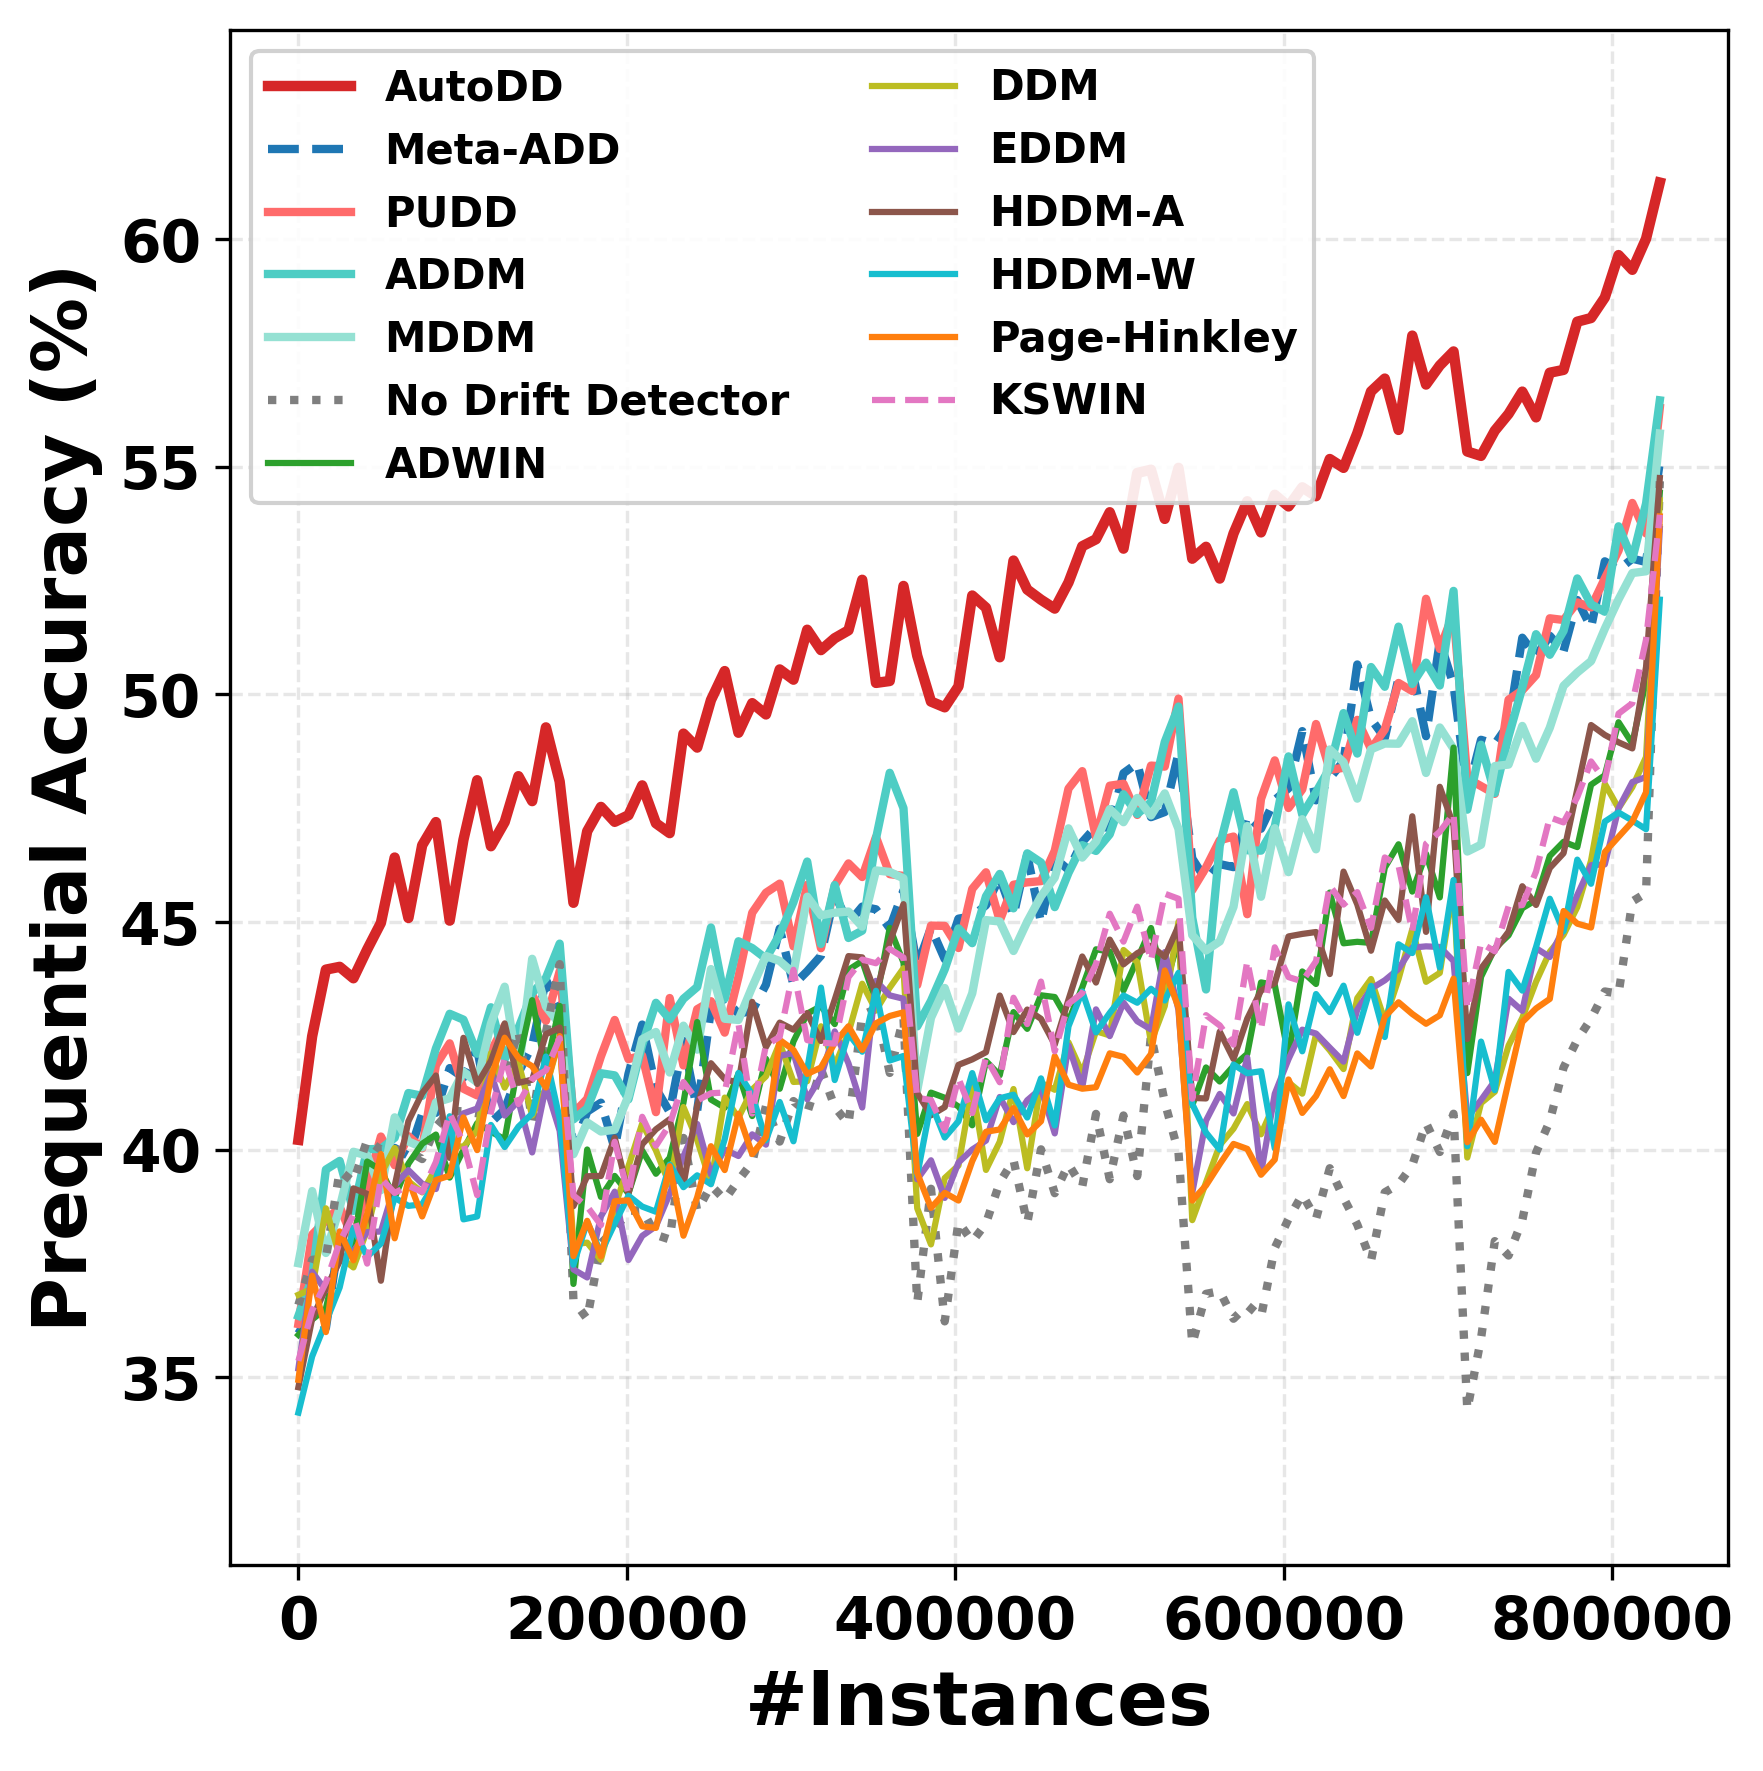
\includegraphics[width=\textwidth]{images/prequential_poker_gaussiannb.png}
        \caption{Poker (GNB)}
    \end{subfigure}
    \hfill
    \begin{subfigure}[b]{0.24\textwidth}
        \centering
        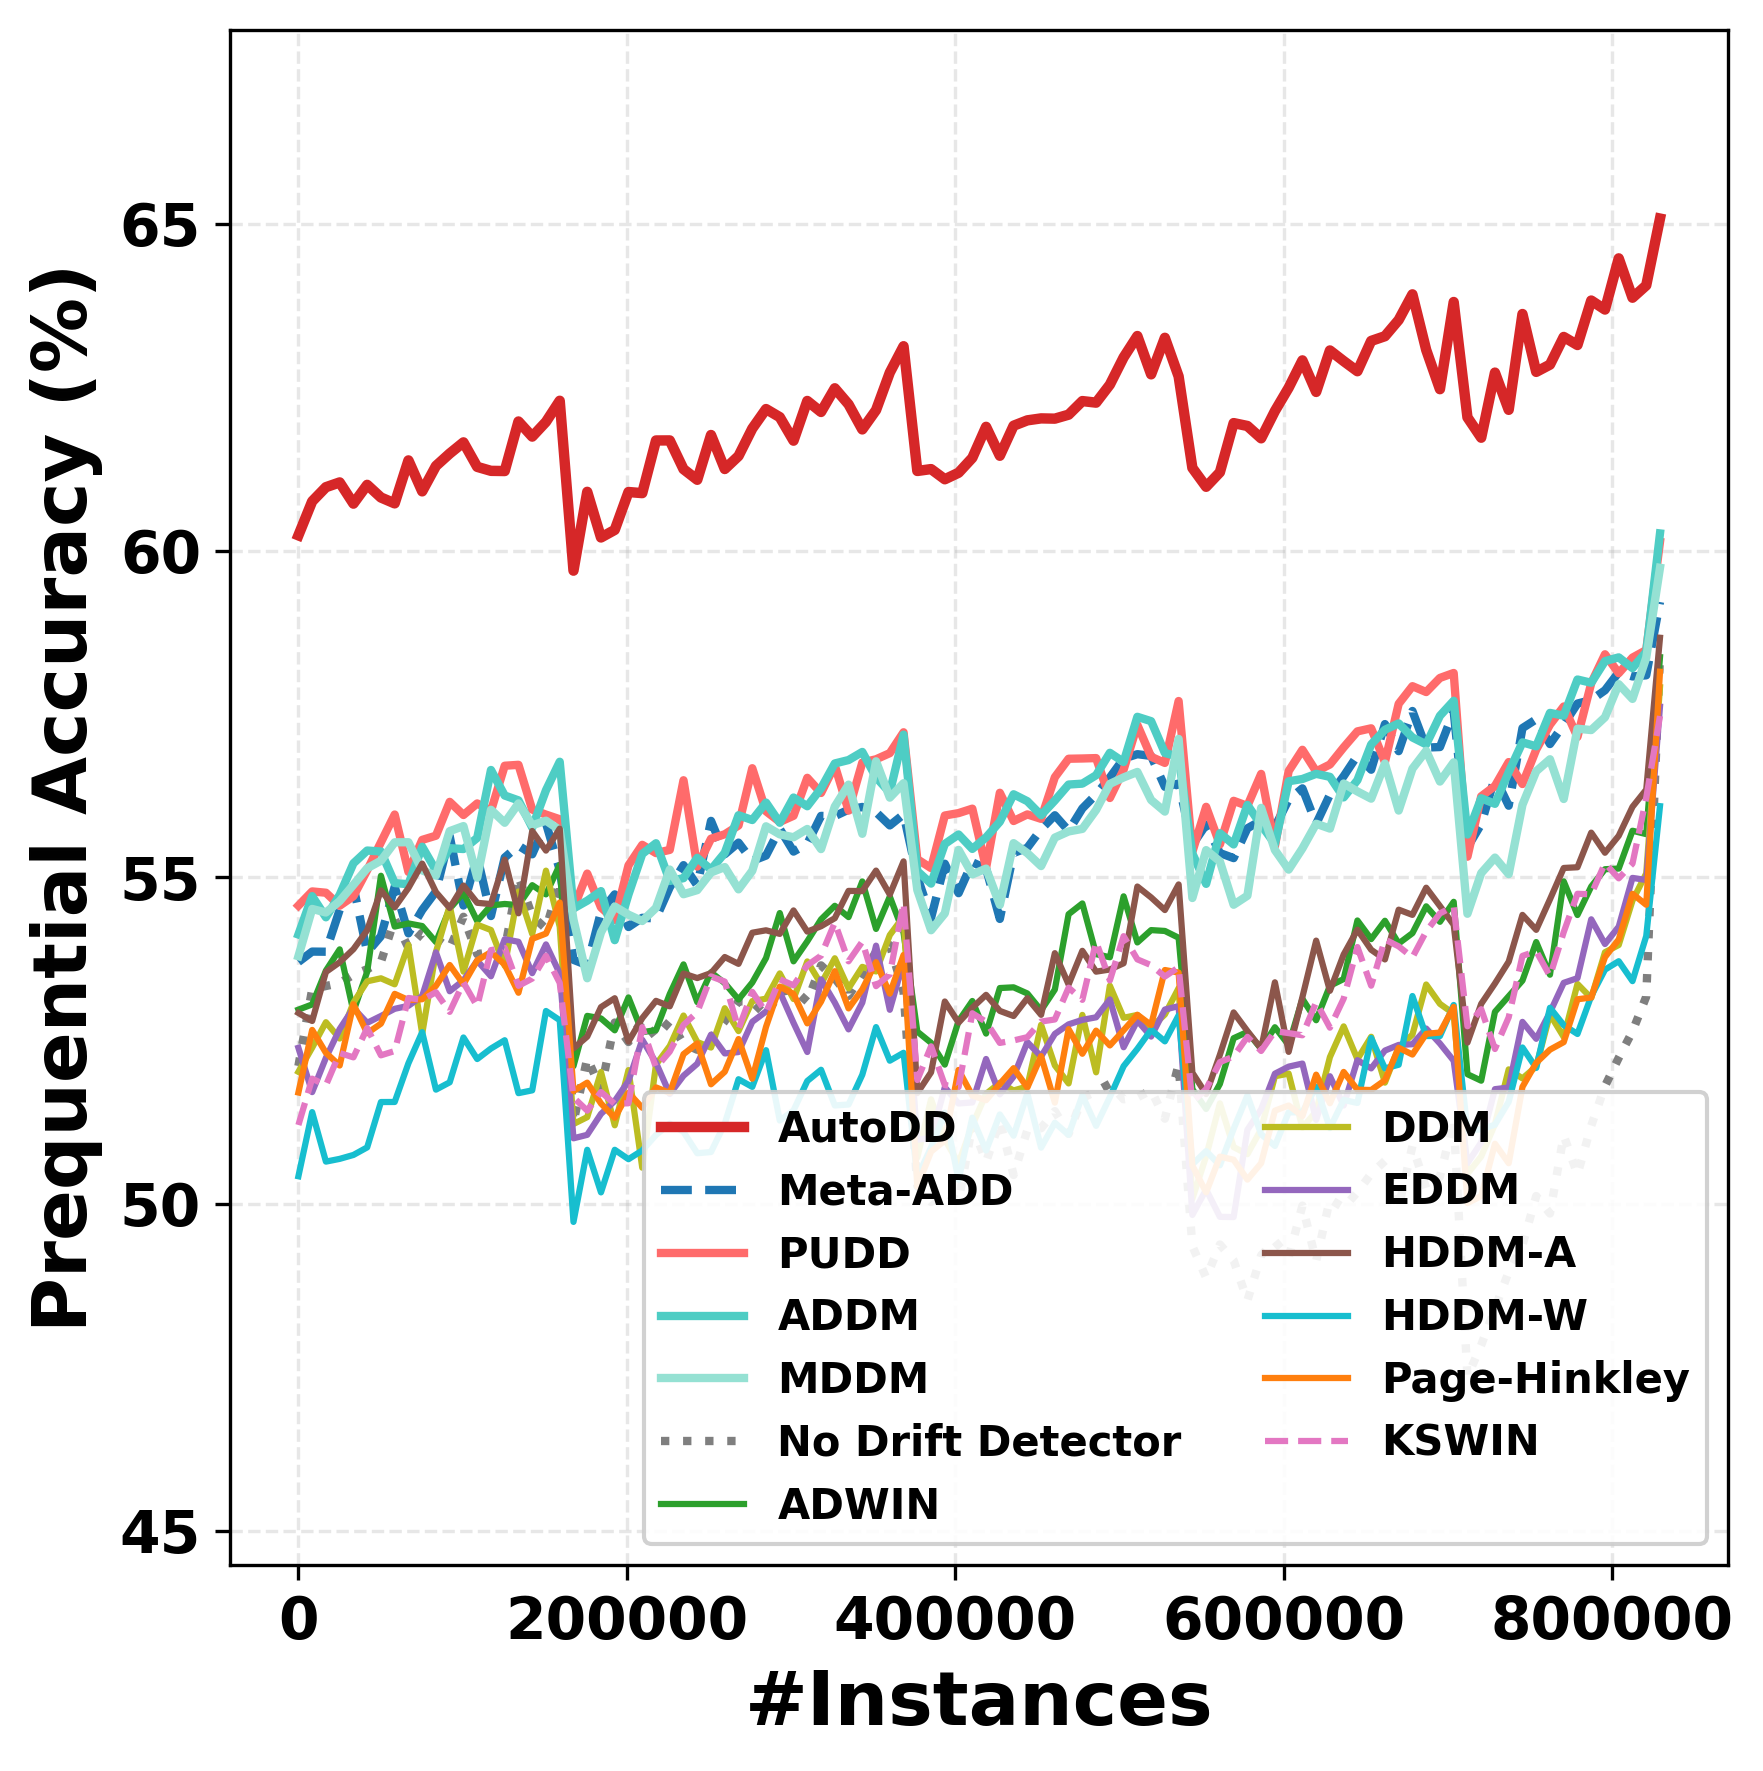
\includegraphics[width=\textwidth]{images/prequential_poker_hat.png}
        \caption{Poker (HAT)}
    \end{subfigure}
    \caption{Prequential accuracy over time. SEA (synthetic) and Poker (real-world) datasets with GaussianNB and HAT base classifiers.}
    \label{fig:prequential}
\end{figure*}

\textbf{Statistical Significance:} To validate the observed performance differences, we conduct statistical significance analysis using GaussianNB as the base classifier. Figure~\ref{fig:cd_diagram} presents the Critical Difference diagram based on the Friedman test with Nemenyi post-hoc analysis at significance level $\alpha=0.05$. AutoDD achieves the best average rank among all methods, demonstrating statistically significant improvements over the baseline detectors. The state-of-the-art methods Meta-ADD, ADDM, PUDD, and MDDM follow in subsequent ranks, while portfolio detectors cluster in middle positions. The No Detector baseline performs worst, confirming that drift detection is essential for streaming data. Connecting bars in the diagram indicate groups of methods that are not statistically different from each other, highlighting that AutoDD's improvements are significant rather than due to random variation.

\begin{figure}[!ht]
    \centering
    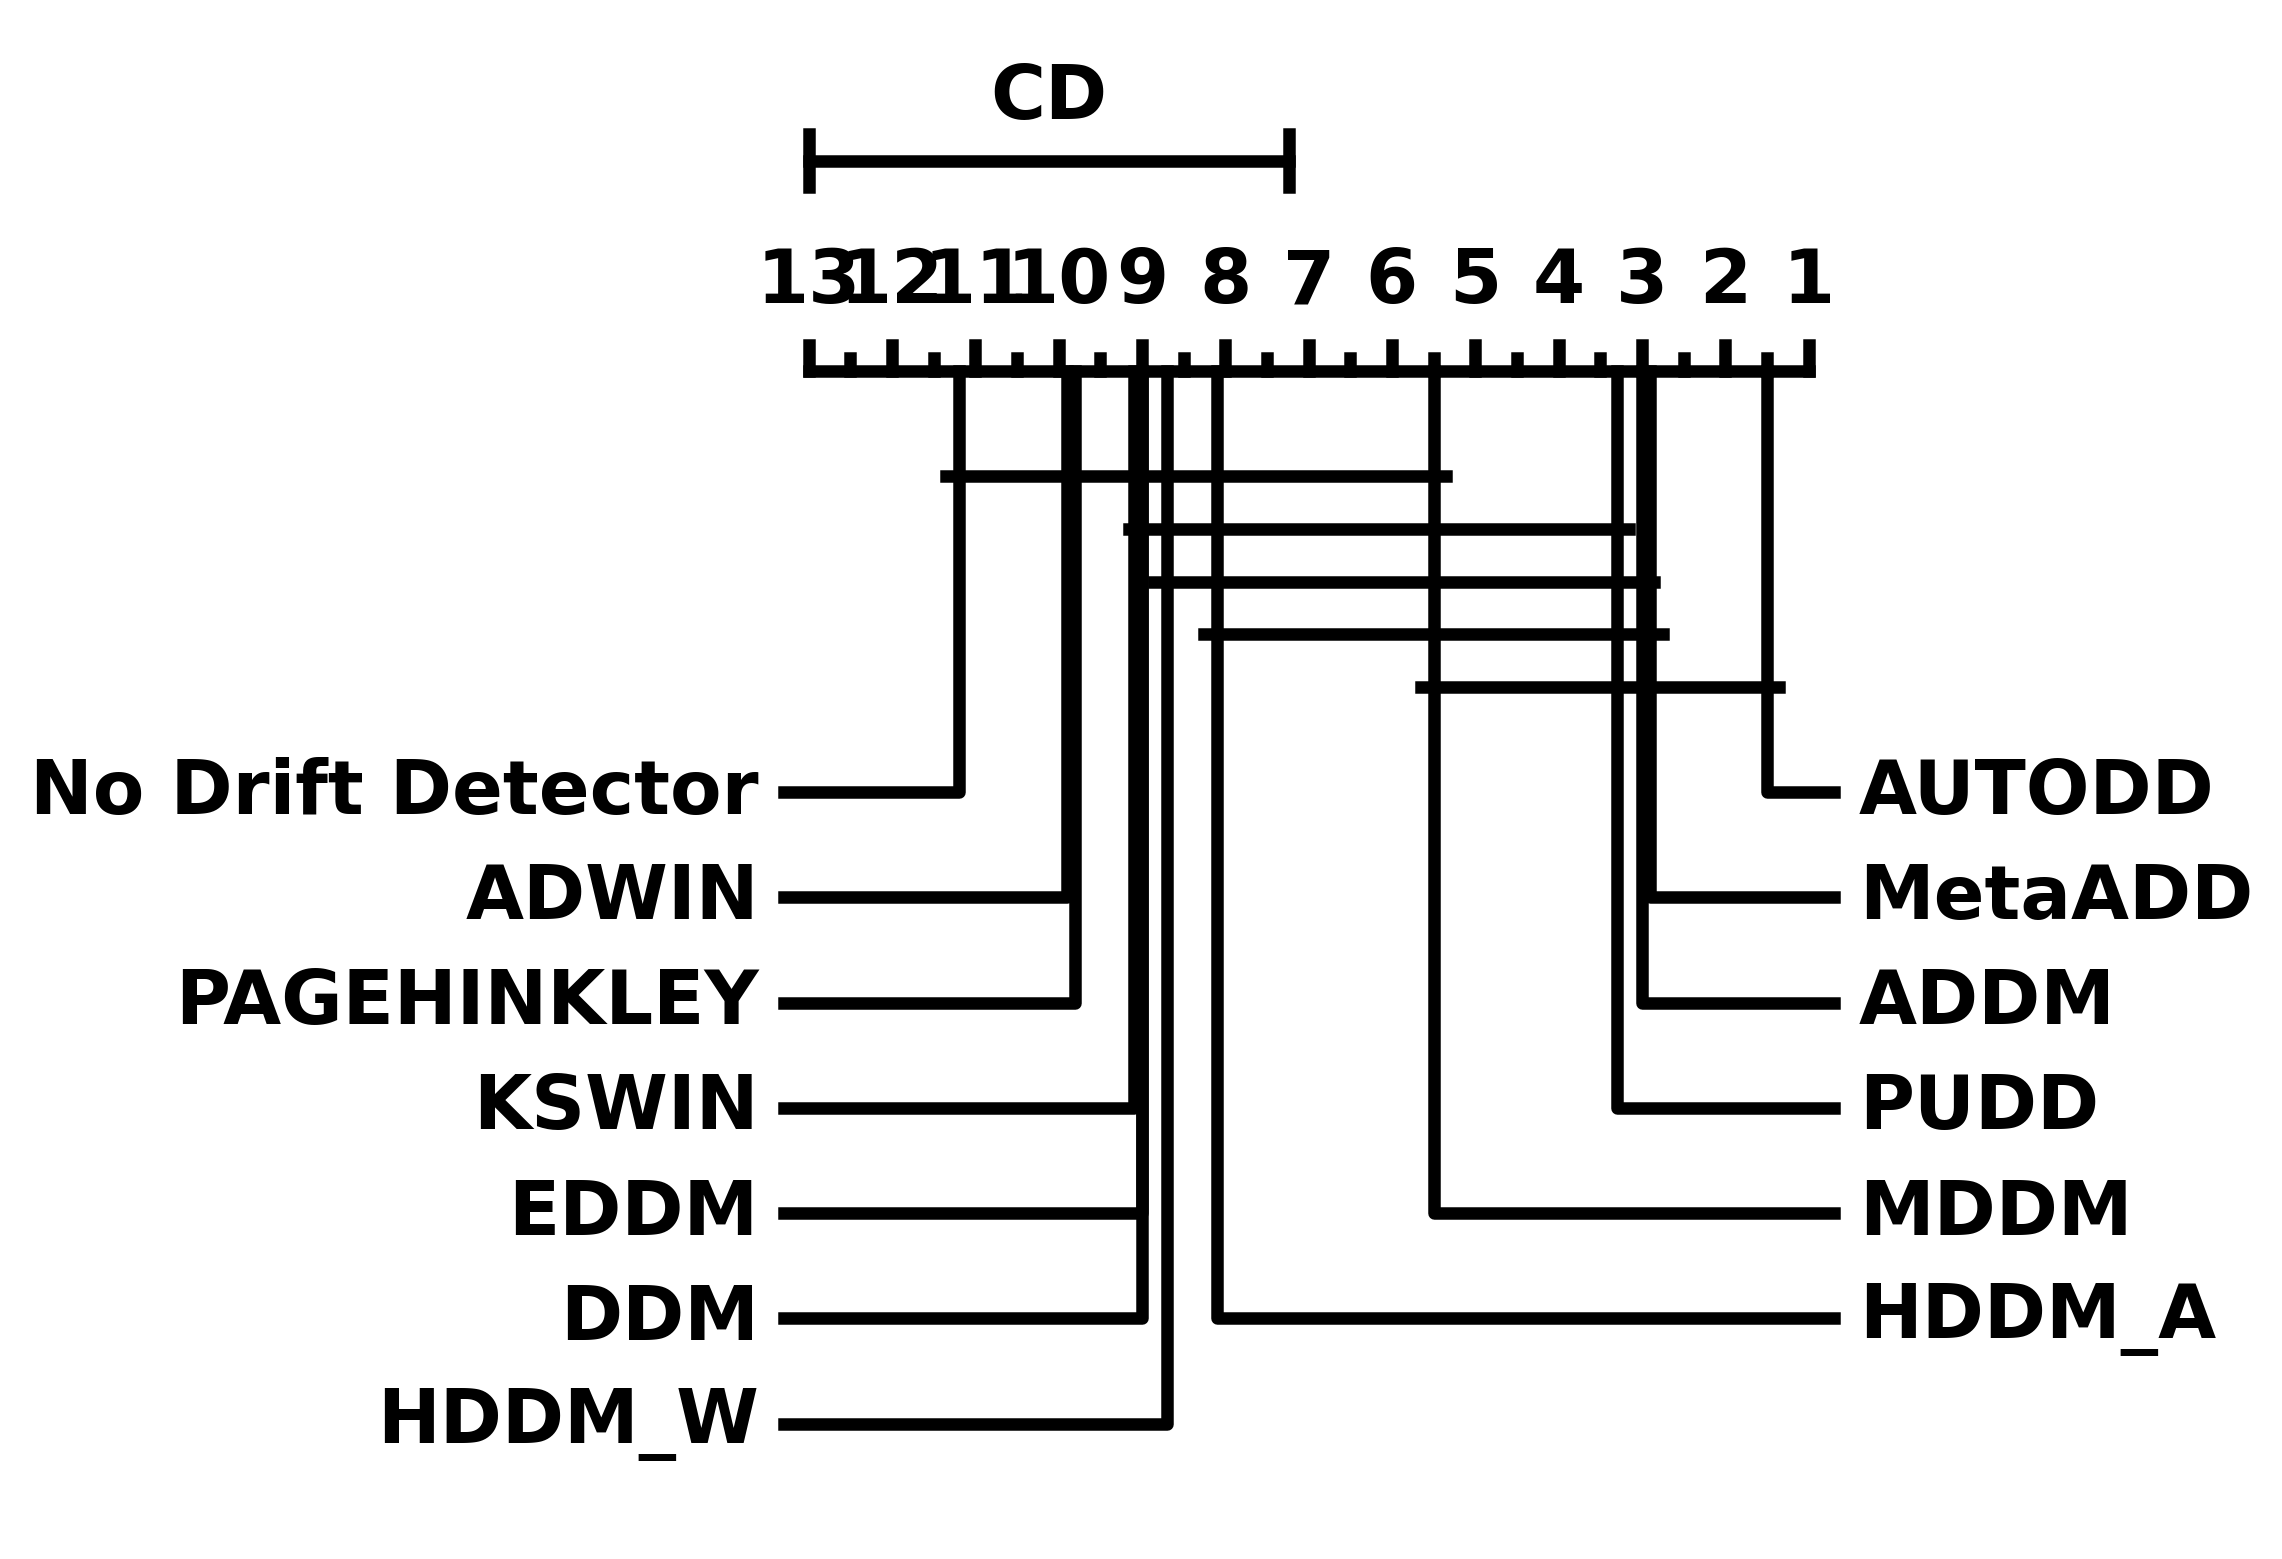
\includegraphics[width=0.75\columnwidth]{images/cd_diagram_gaussiannb.png}
    \caption{Critical Difference diagram with connecting bars indicating statistically equivalent methods.}
    \label{fig:cd_diagram}
\end{figure}


\textbf{Ablation Study:} To understand the contribution of each component, we systematically remove AutoDD components and evaluate the impact on performance using GaussianNB as the base classifier. Table~\ref{tab:ablation} presents results averaged across all ten datasets. The hierarchical selection mechanism proves critical for AutoDD's performance. Removing Level 1 LinUCB detector selection and replacing it with random selection causes the largest performance drop, reducing accuracy from 80.5\% to 62.5\%, an 18.0\% decrease. This substantial degradation confirms that intelligent detector-stream matching is essential for effective drift detection. Removing Level 2 Thompson Sampling hyperparameter configuration reduces accuracy to 75.3\%, demonstrating that adaptive tuning contributes meaningfully beyond fixed default configurations. All three meta-feature categories contribute substantially to the overall performance. Statistical features have the largest impact, with their removal reducing accuracy by 9.4\%. Stationarity features contribute 7.1\% to performance, while temporal features account for 6.4\%. Figure~\ref{fig:detector_selection} visualizes AutoDD's adaptive behavior on the Hyperplane dataset, showing how the framework dynamically switches between detectors in response to changing stream conditions and drift events.

\begin{table}[!ht]
\centering
\caption{Ablation study results (all 10 datasets)}
\label{tab:ablation}
\begin{tabular}{lccc}
\toprule
\textbf{Configuration} & \textbf{Accuracy} & \textbf{F1} & \textbf{$\Delta$Acc} \\
\midrule
Full AutoDD & \textbf{80.5\%} & \textbf{0.64} & -- \\
w/o Temporal & 74.2\% & 0.59 & -6.4\% \\
w/o Statistical & 71.2\% & 0.57 & -9.4\% \\
w/o Stationarity & 73.5\% & 0.59 & -7.1\% \\
w/o LinUCB (Level 1) & 62.5\% & 0.50 & -18.0\% \\
w/o Thompson (Level 2) & 75.3\% & 0.60 & -5.2\% \\
\bottomrule
\end{tabular}
\end{table}

% \begin{figure}[!ht]
%     \centering
%     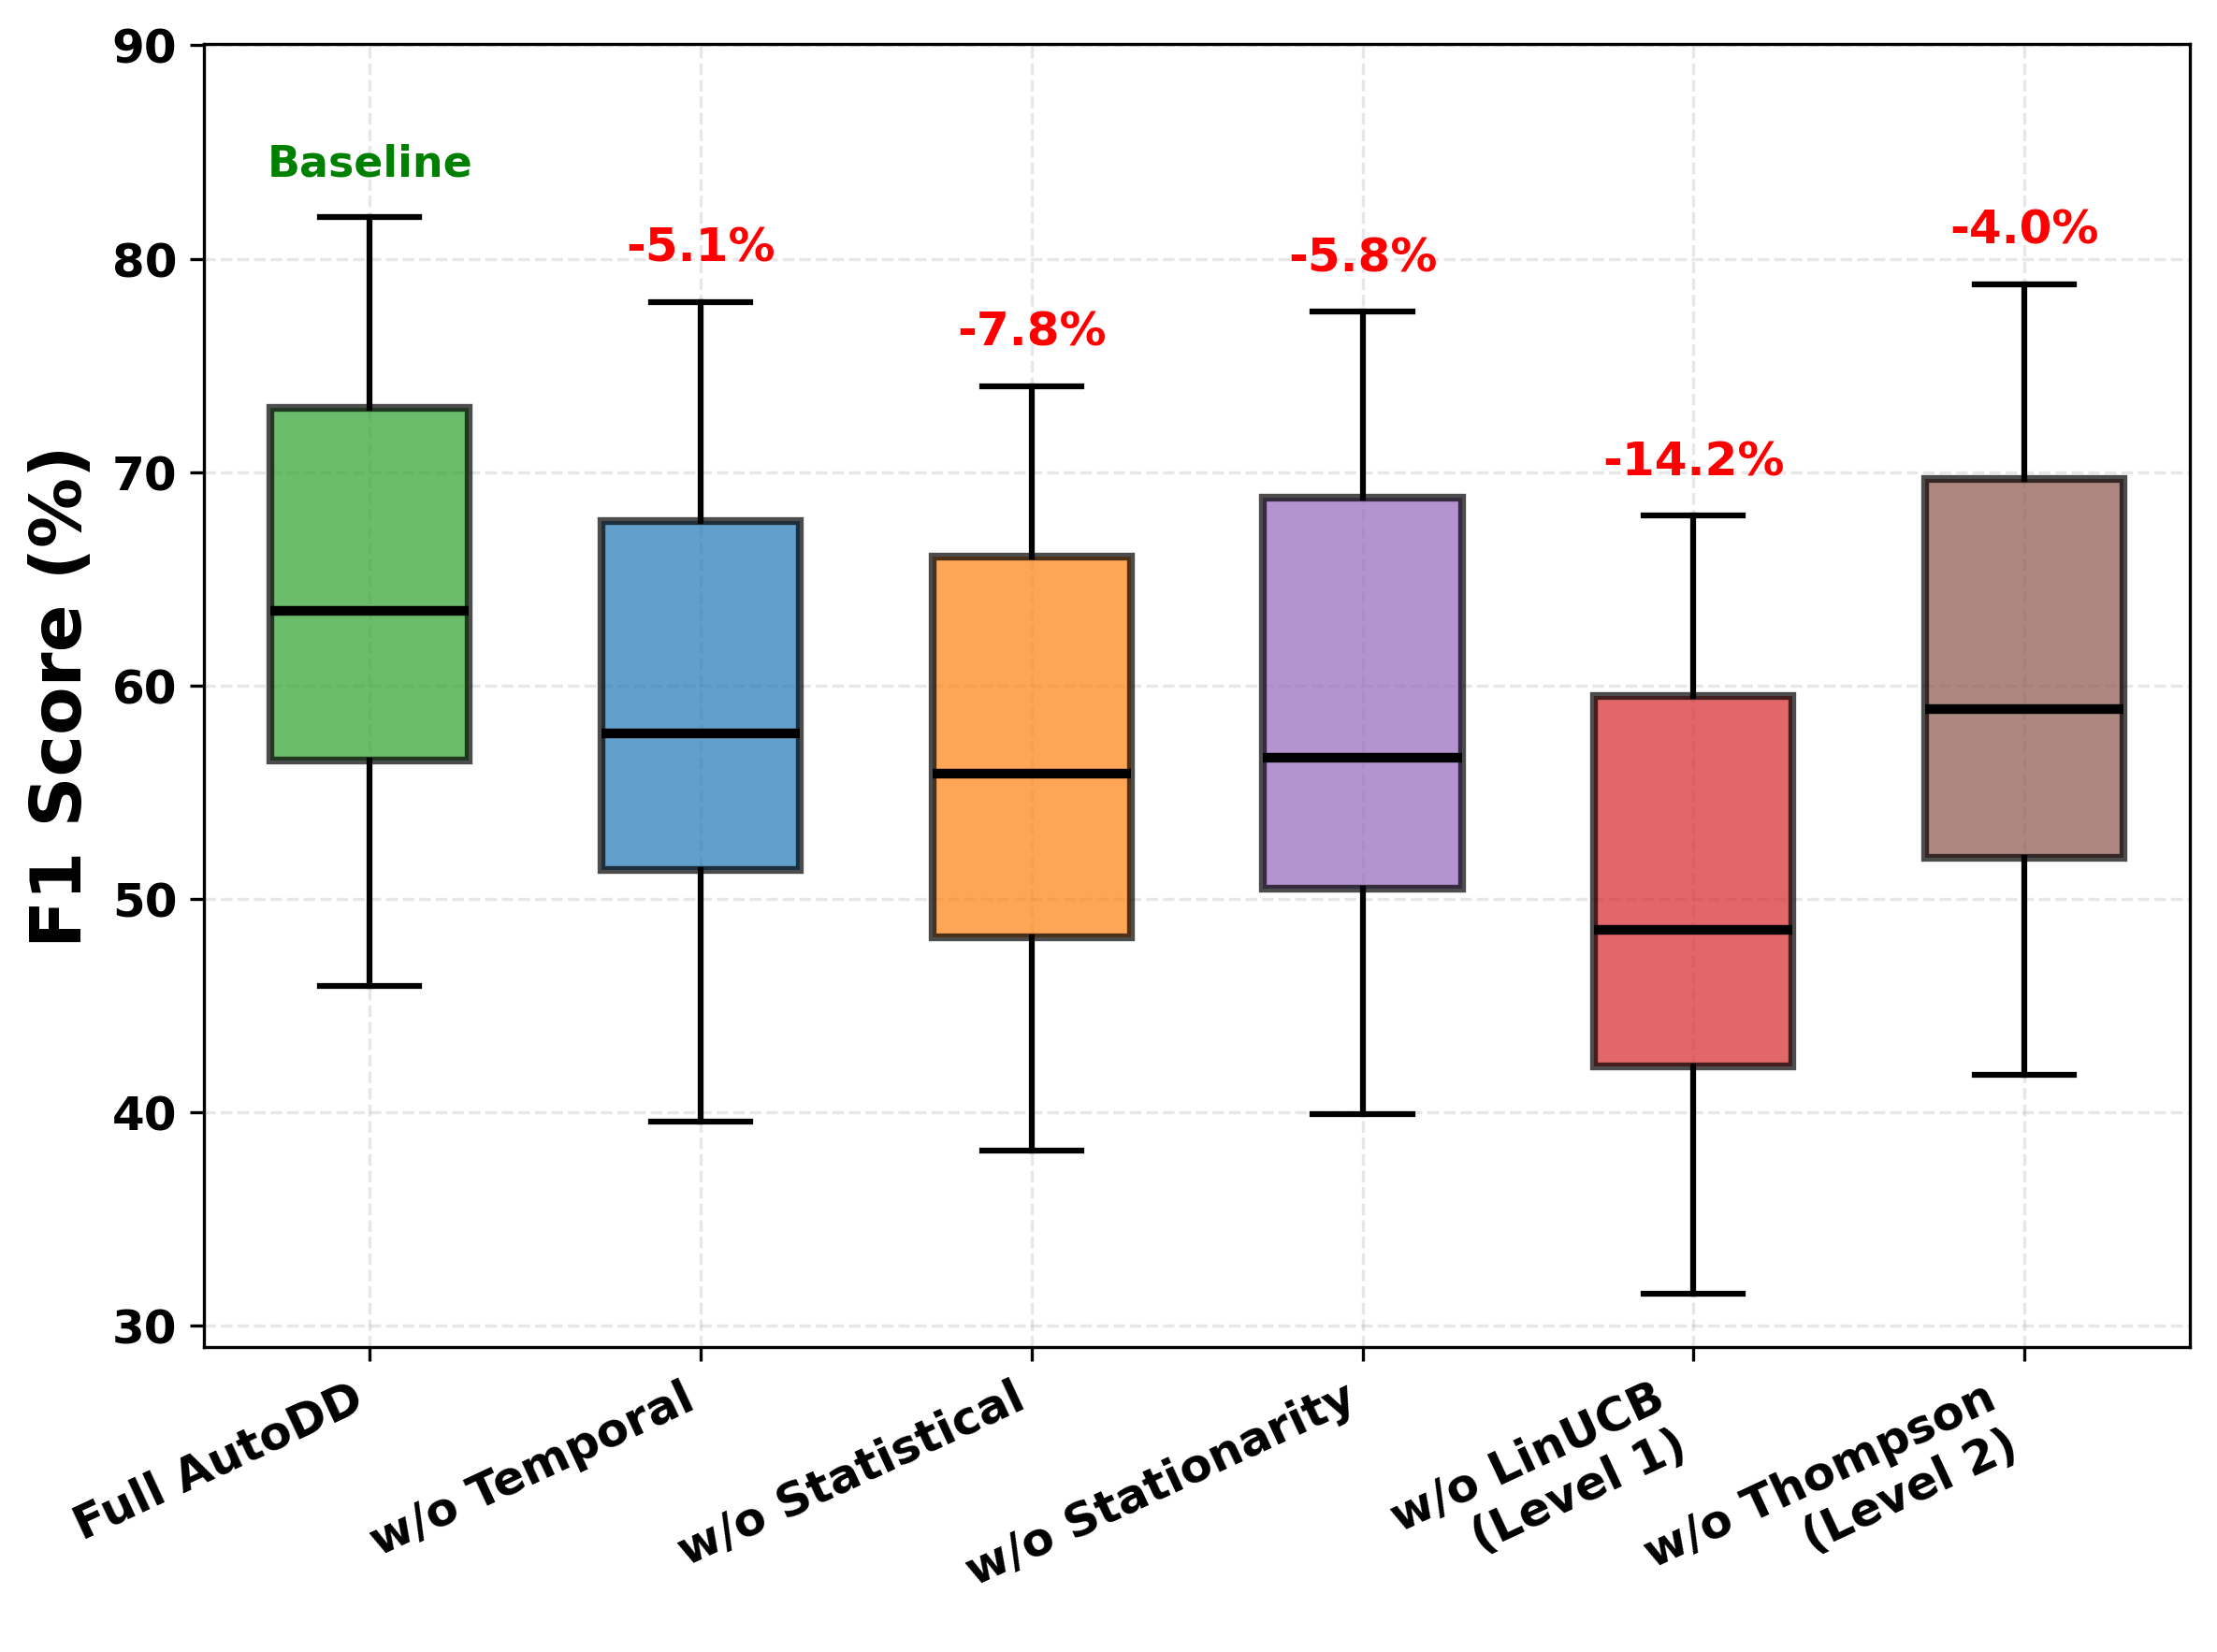
\includegraphics[width=\columnwidth]{images/ablation_f1.png}
%     \caption{Ablation study: F1-score comparison across configurations.}
%     \label{fig:ablation}
% \end{figure}


% \begin{table}[!ht]
% \centering
% \caption{Detector selection frequency (\%) by drift type}
% \label{tab:selection}
% \begin{tabular}{lcccc}
% \toprule
% \textbf{Detector} & \textbf{Sudden} & \textbf{Gradual} & \textbf{Increm.} & \textbf{Normal} \\
% \midrule
% ADWIN & 68.2 & 12.4 & 7.8 & 16.1 \\
% DDM & 15.4 & 8.1 & 5.7 & 13.3 \\
% EDDM & 3.8 & 22.4 & 8.7 & 9.3 \\
% HDDM-A & 2.1 & 7.8 & 17.3 & 6.8 \\
% HDDM-W & 1.2 & 3.8 & 11.8 & 4.5 \\
% Page-Hinkley & 0.9 & 0.5 & 0.5 & 30.6 \\
% KSWIN & 8.5 & 45.1 & 48.3 & 19.4 \\
% \bottomrule
% \end{tabular}
% \end{table}

\begin{figure}[!ht]
    \centering
    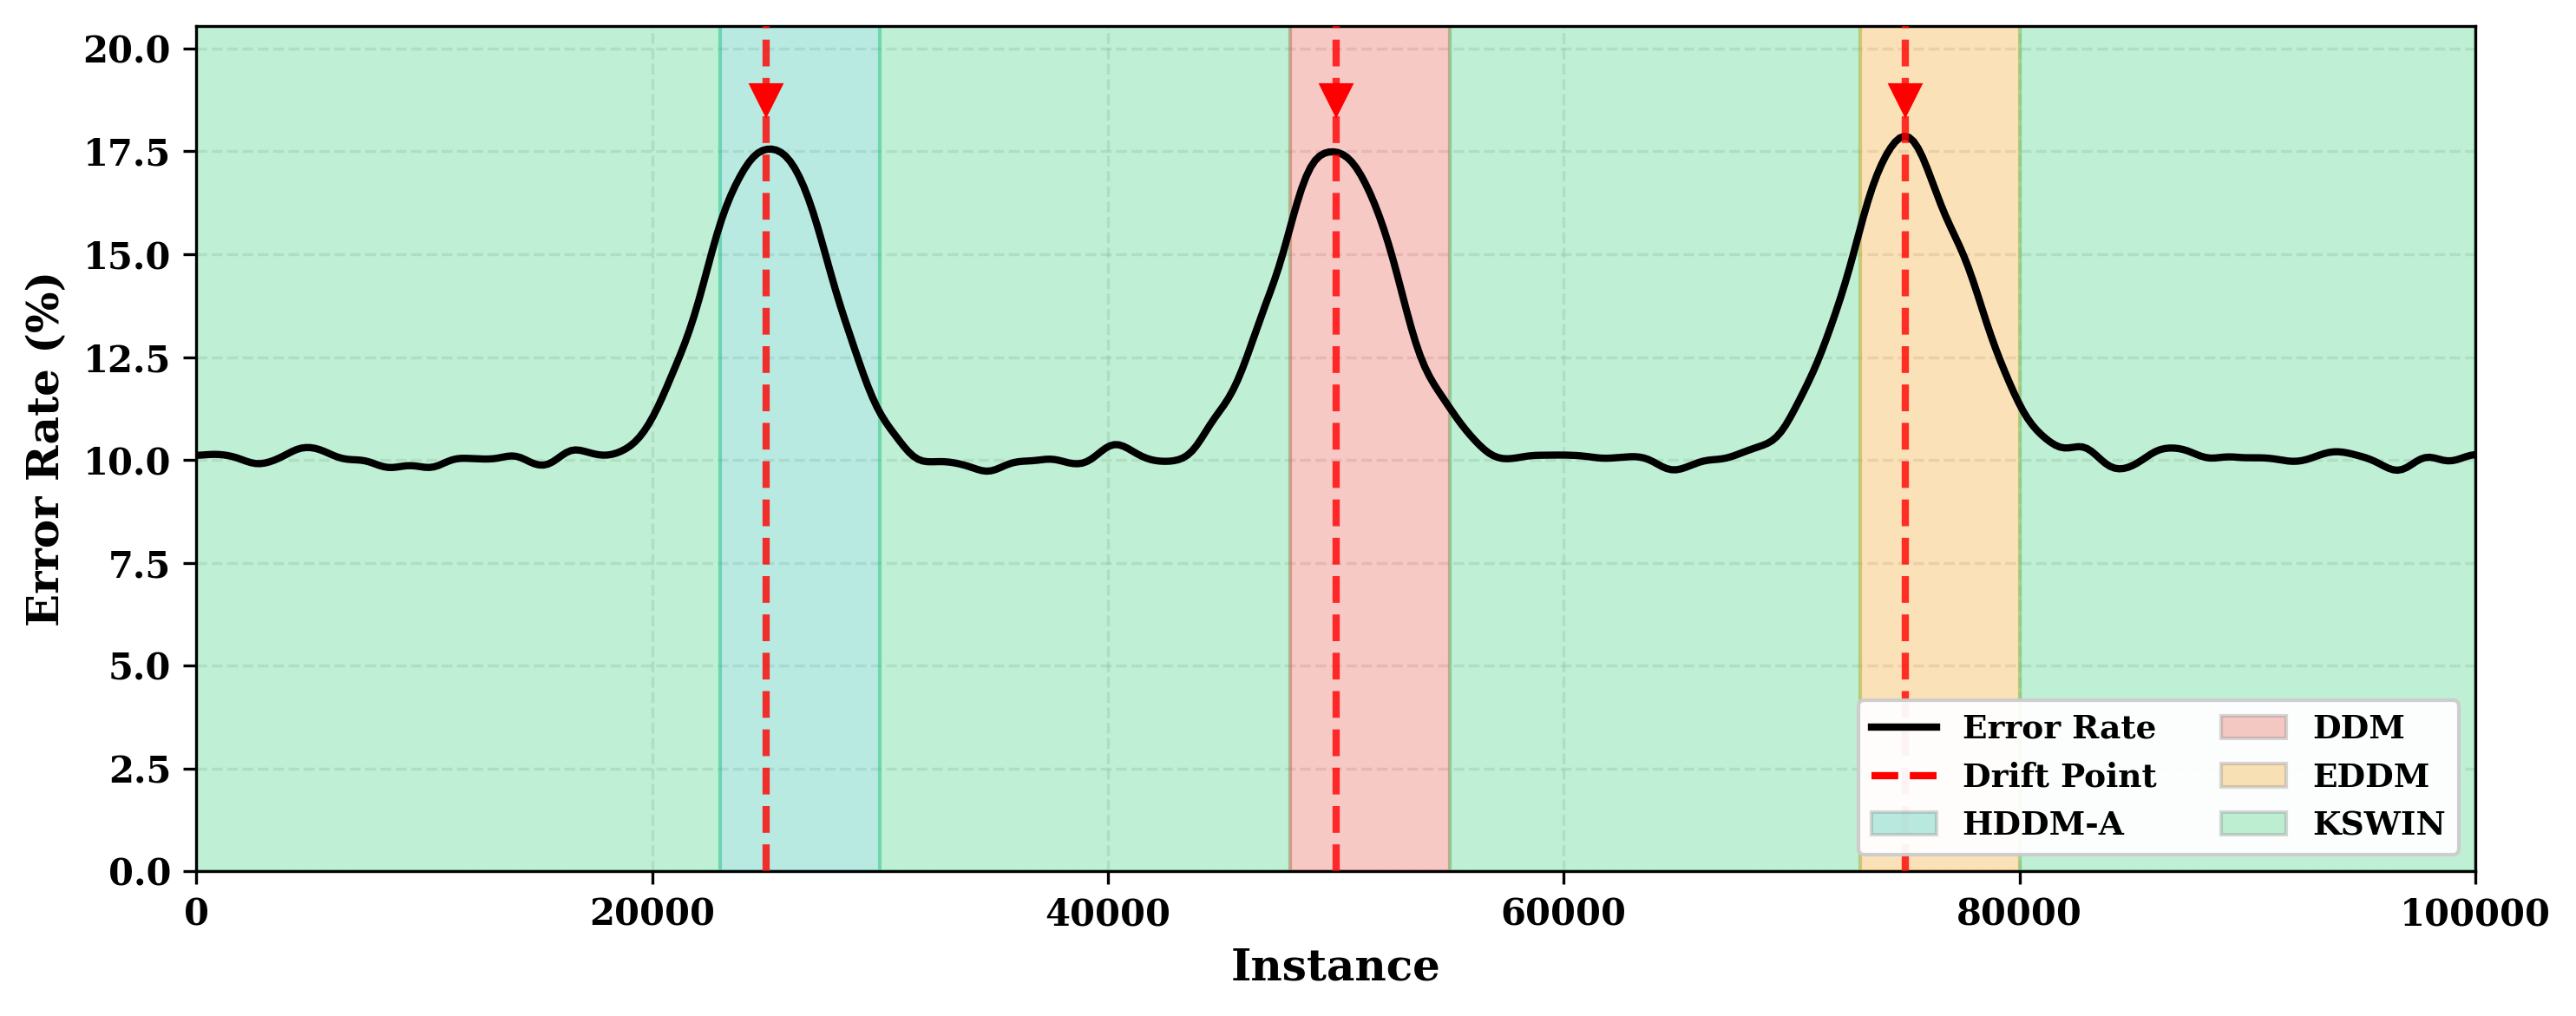
\includegraphics[width=0.75\columnwidth]{images/detector_selection_hyp.png}
    \caption{Detector selection on Hyperplane stream showing active detectors, error rate, and drift points.}
    \label{fig:detector_selection}
\end{figure}

\textbf{Sensitivity Study:} We analyze AutoDD's sensitivity to key hyperparameters using GaussianNB as the base classifier (Figure~\ref{fig:sensitivity}). The optimal window size of $w=100$ achieves 92.6\% selection accuracy, balancing statistical stability with drift responsiveness. Smaller windows suffer from high variance, while larger windows cause delayed drift response. For the exploration parameter, $\alpha=1.0$ achieves best performance, with lower values causing exploitation bias and higher values leading to excessive exploration. The regularization parameter $\lambda$ shows robust performance across the range from 0.5 to 2.0, with $\lambda=1.0$ being optimal. This stability indicates that AutoDD is not overly sensitive to hyperparameter choices around the recommended defaults.

% \begin{table}[!ht]
% \centering
% \caption{Selection accuracy (\%) vs. window size and meta-features}
% \label{tab:metafeatures}
% \resizebox{\columnwidth}{!}{%
% \begin{tabular}{lccccc}
% \toprule
% \textbf{Meta-Features} & $w=25$ & $w=50$ & $w=100$* & $w=150$ & $w=200$ \\
% \midrule
% Statistical only & 62.3 & 69.0 & 75.0 & 73.5 & 72.5 \\
% Stationarity only & 64.9 & 71.5 & 79.3 & 77.9 & 76.2 \\
% Temporal only & 69.9 & 77.2 & 84.2 & 82.9 & 80.8 \\
% All (15 features) & 78.1 & 85.5 & \textbf{92.6} & 91.0 & 88.4 \\
% \bottomrule
% \multicolumn{6}{l}{\small * Optimal window size}
% \end{tabular}%
% }
% \end{table}

\begin{figure}[!ht]
    \centering
    \begin{subfigure}[b]{0.32\columnwidth}
        \centering
        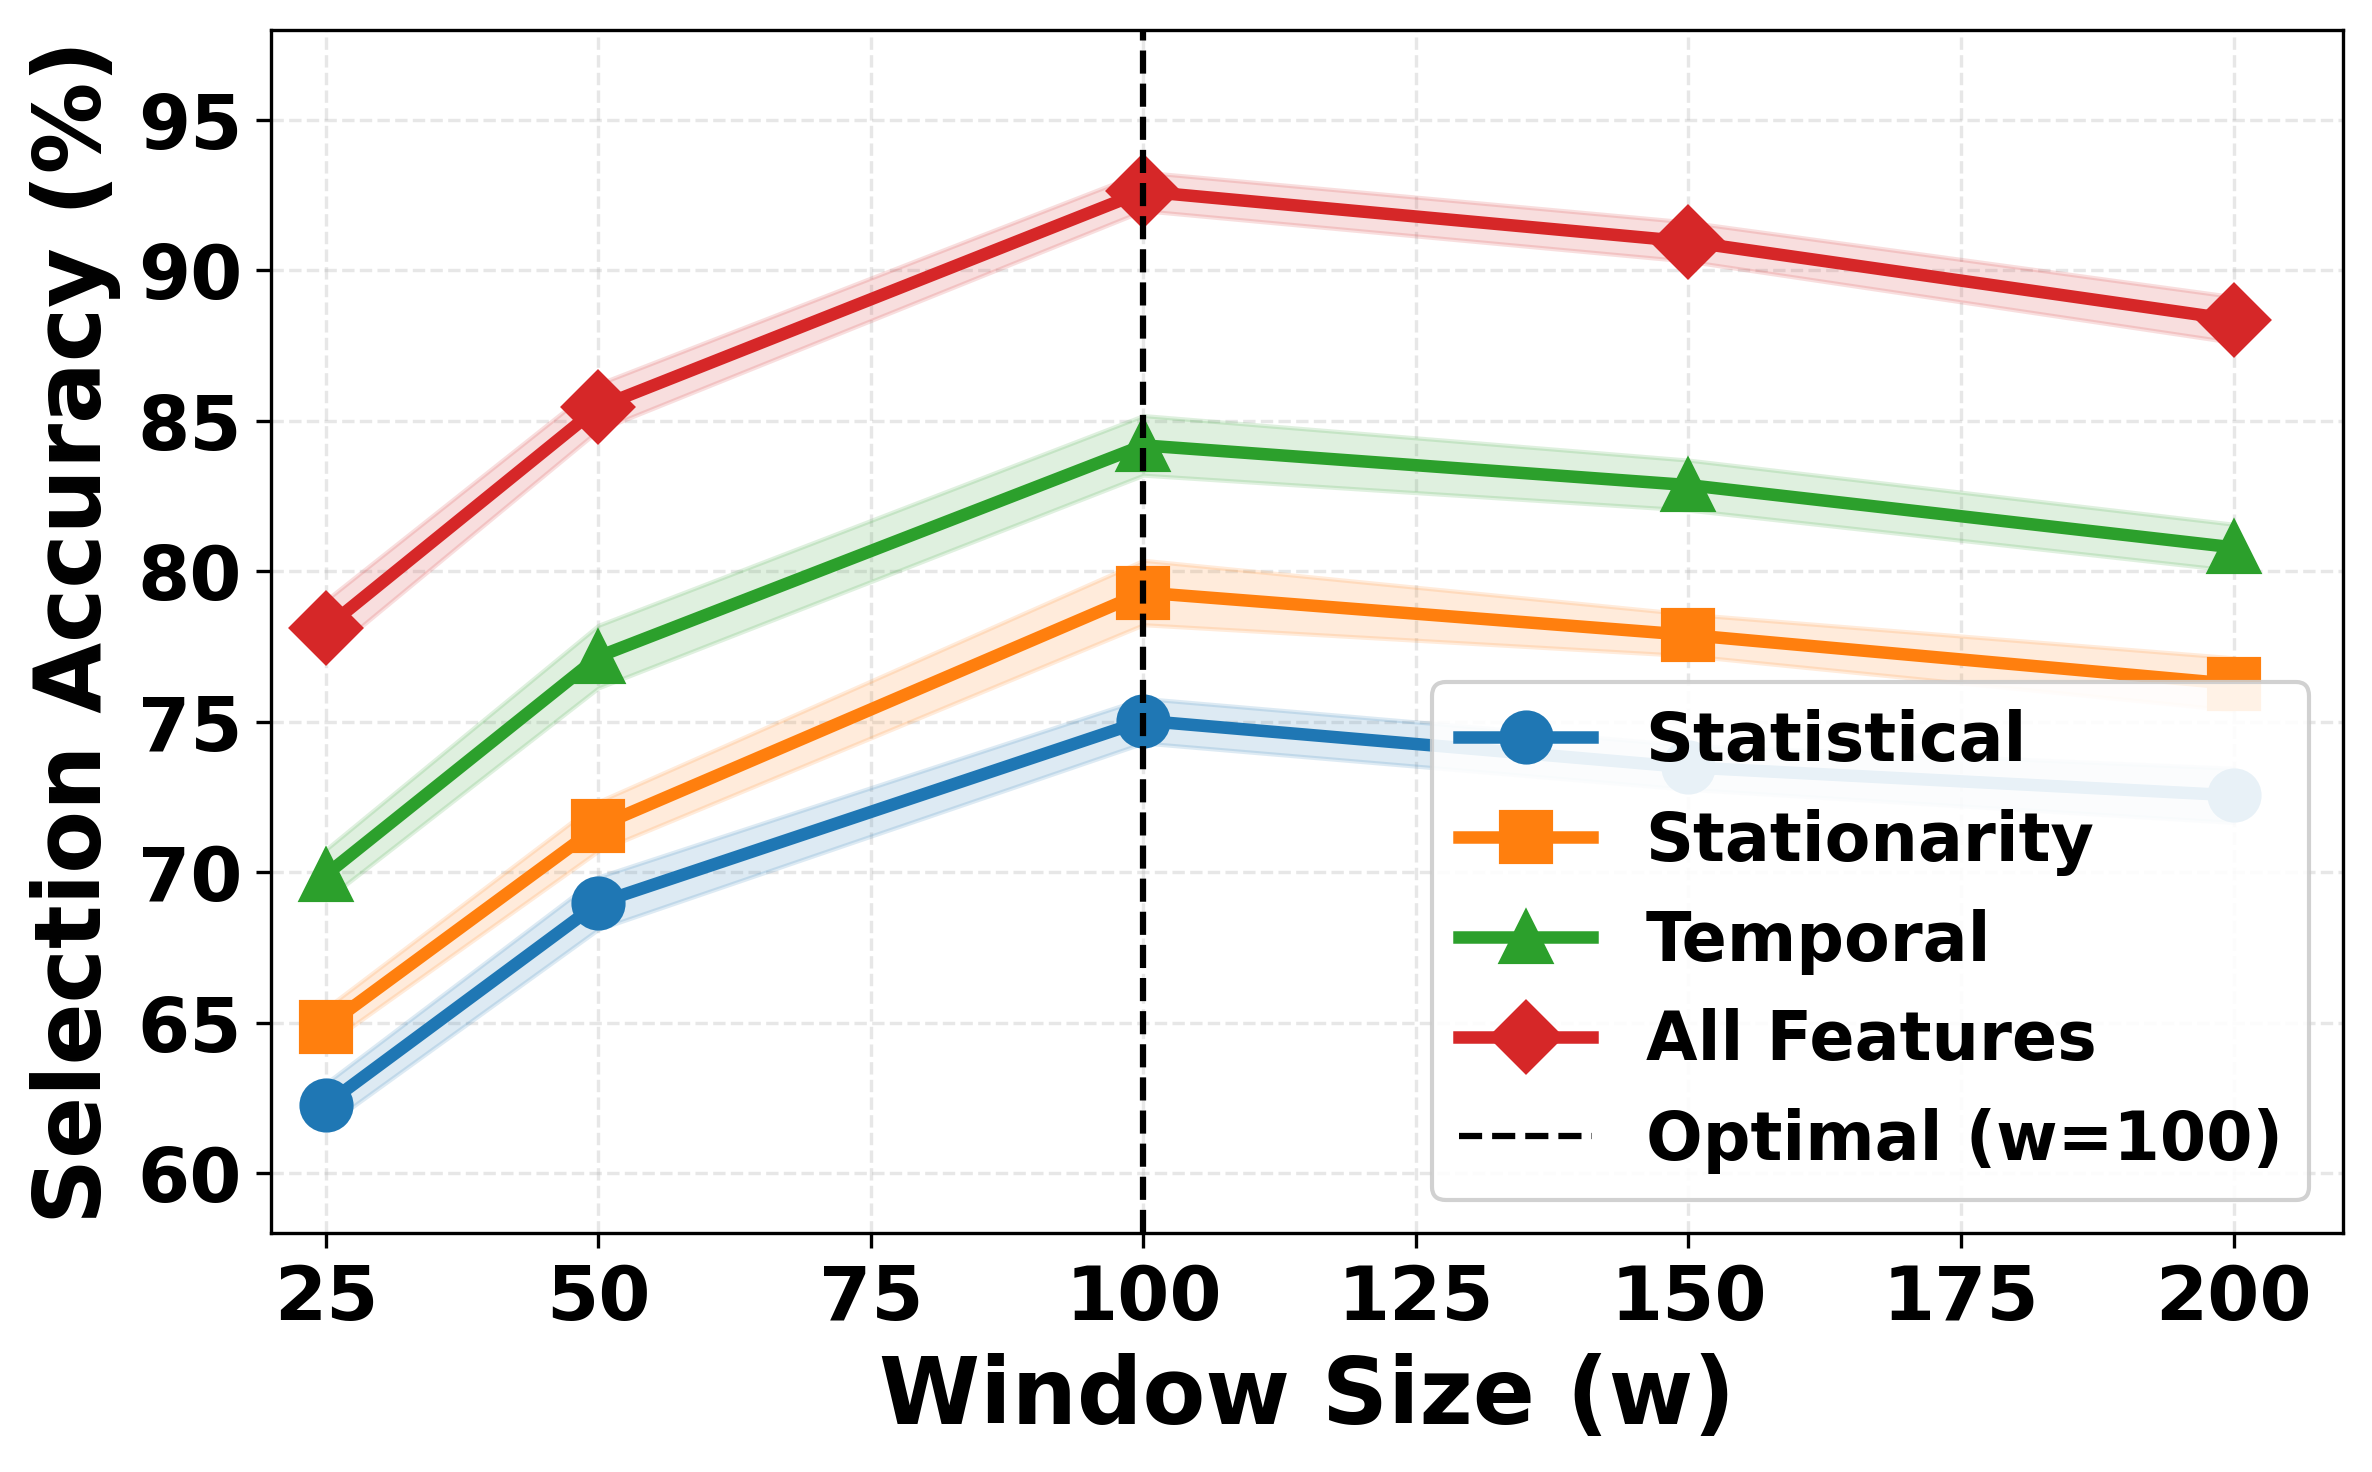
\includegraphics[width=\textwidth]{images/window_sensitivity.png}
        \caption{Window size $w$}
        \label{fig:window_sensitivity}
    \end{subfigure}
    \hfill
    \begin{subfigure}[b]{0.32\columnwidth}
        \centering
        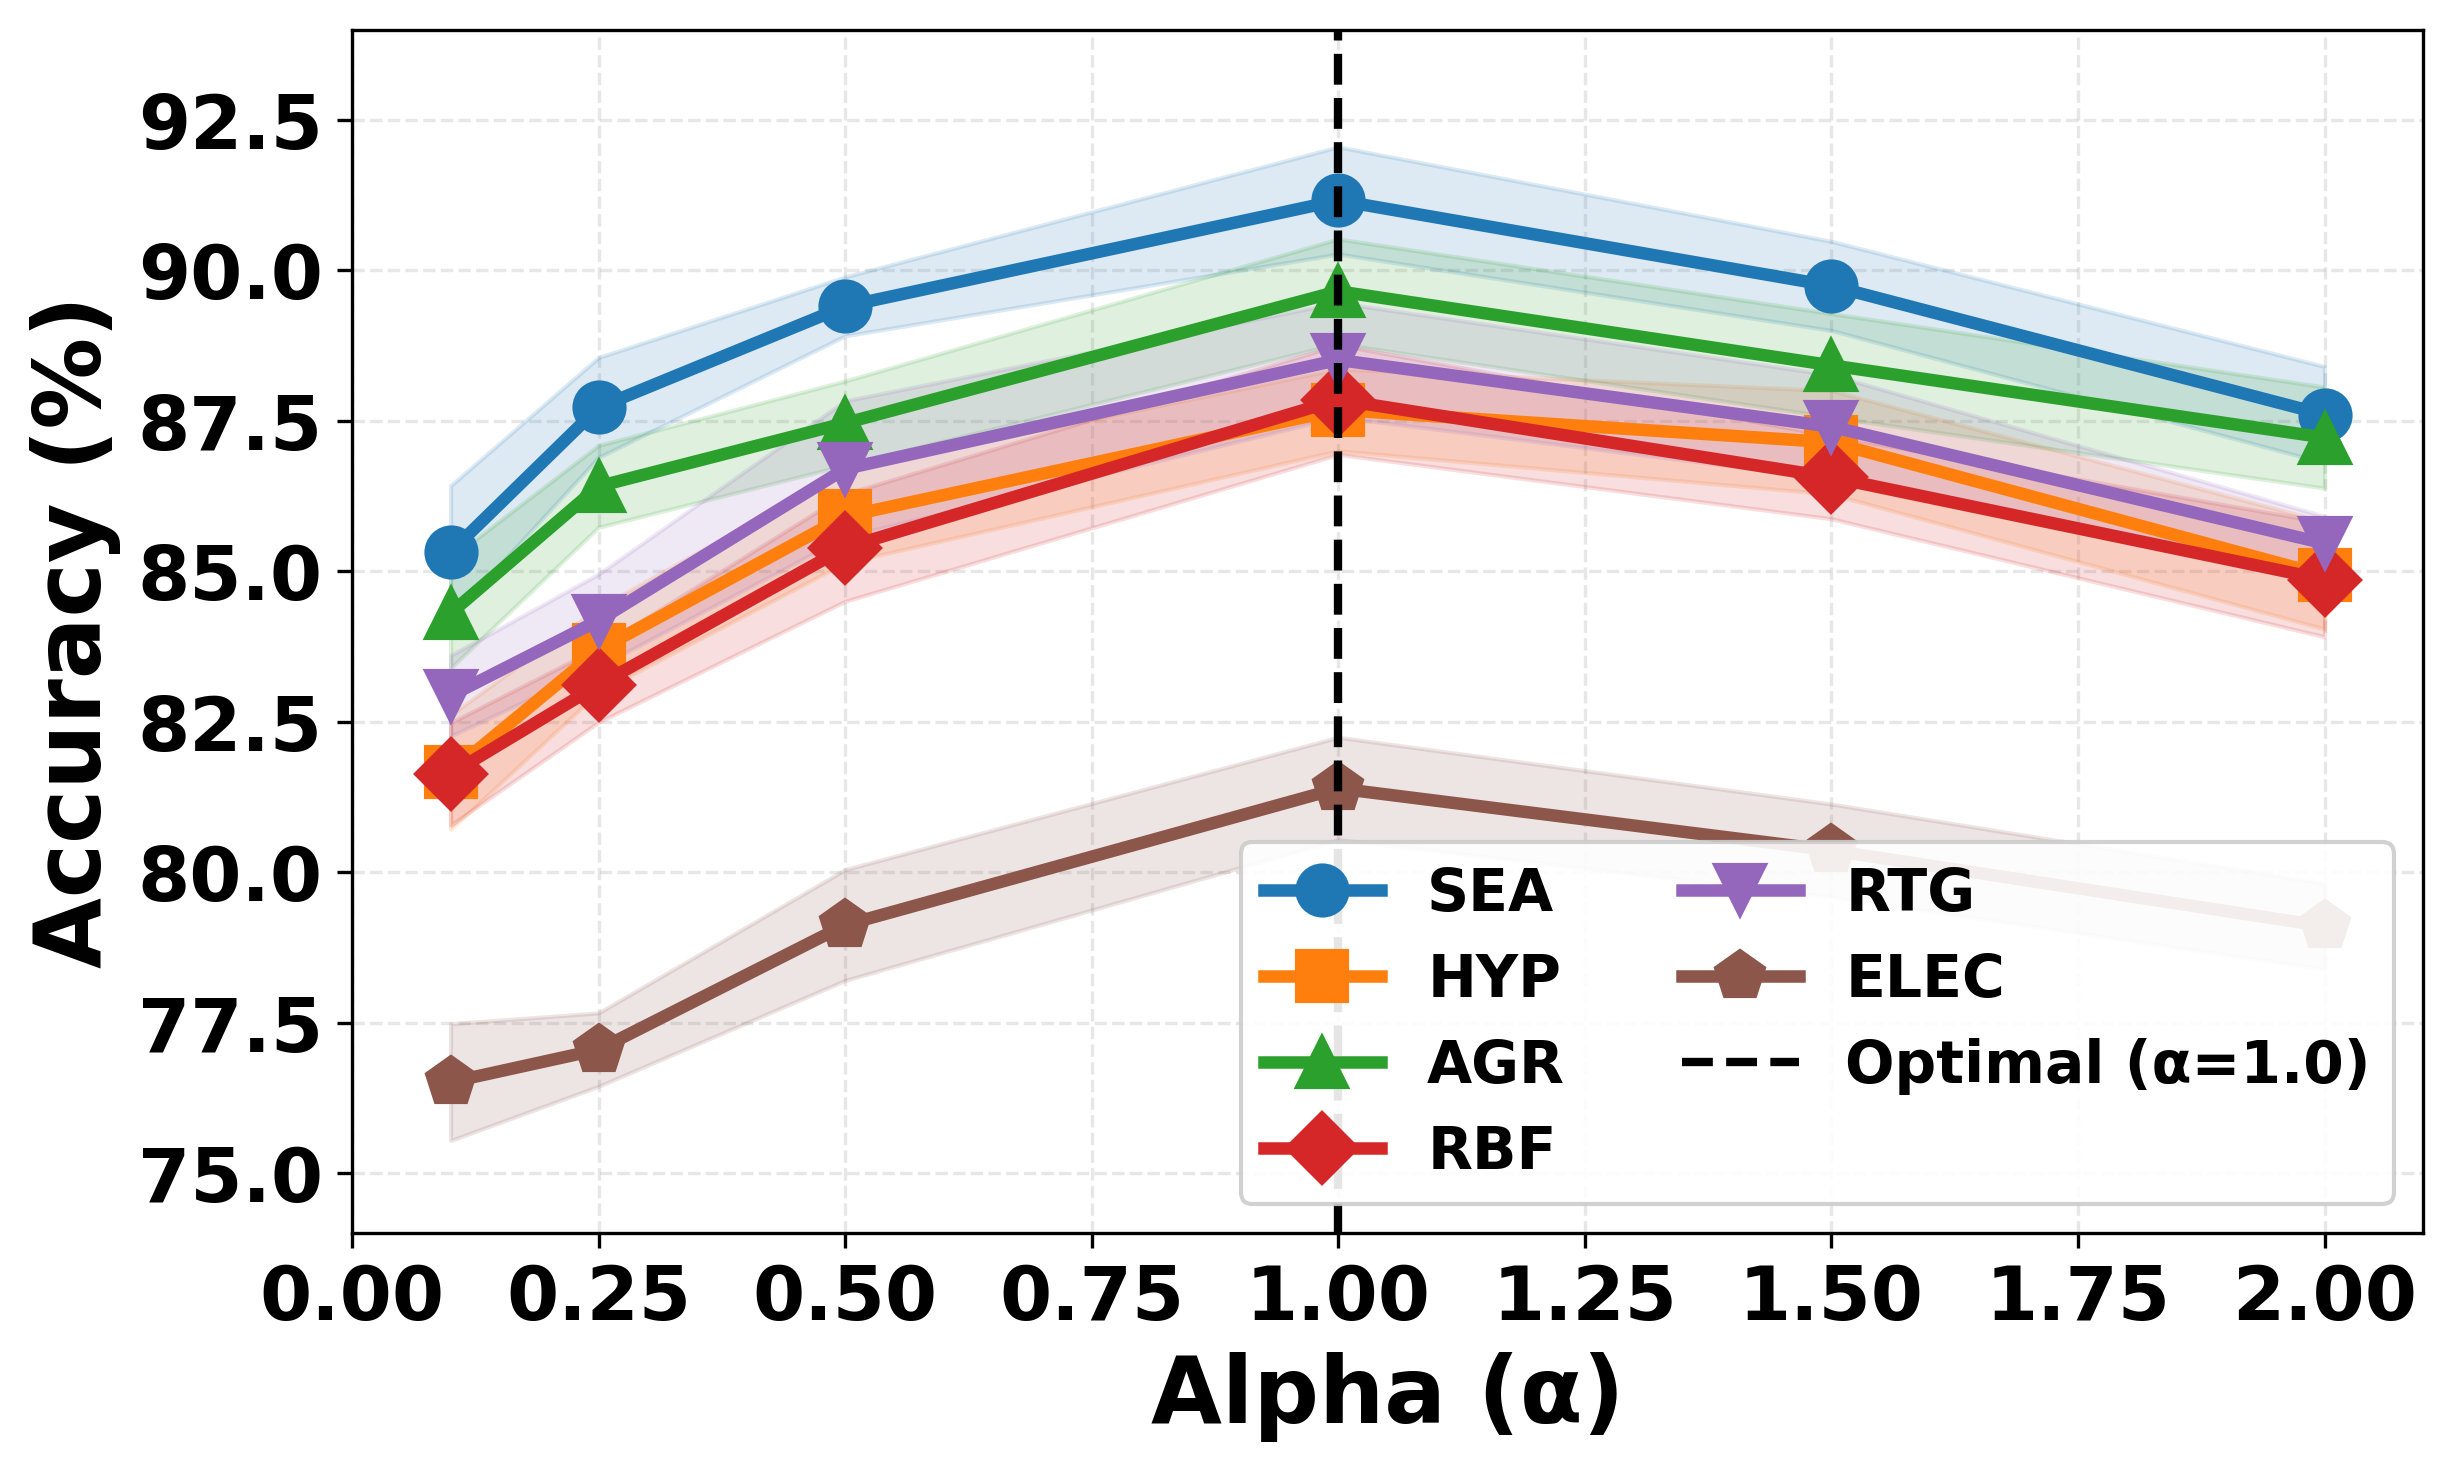
\includegraphics[width=\textwidth]{images/alpha_sensitivity.png}
        \caption{Exploration $\alpha$}
        \label{fig:alpha_sensitivity}
    \end{subfigure}
    \hfill
    \begin{subfigure}[b]{0.32\columnwidth}
        \centering
        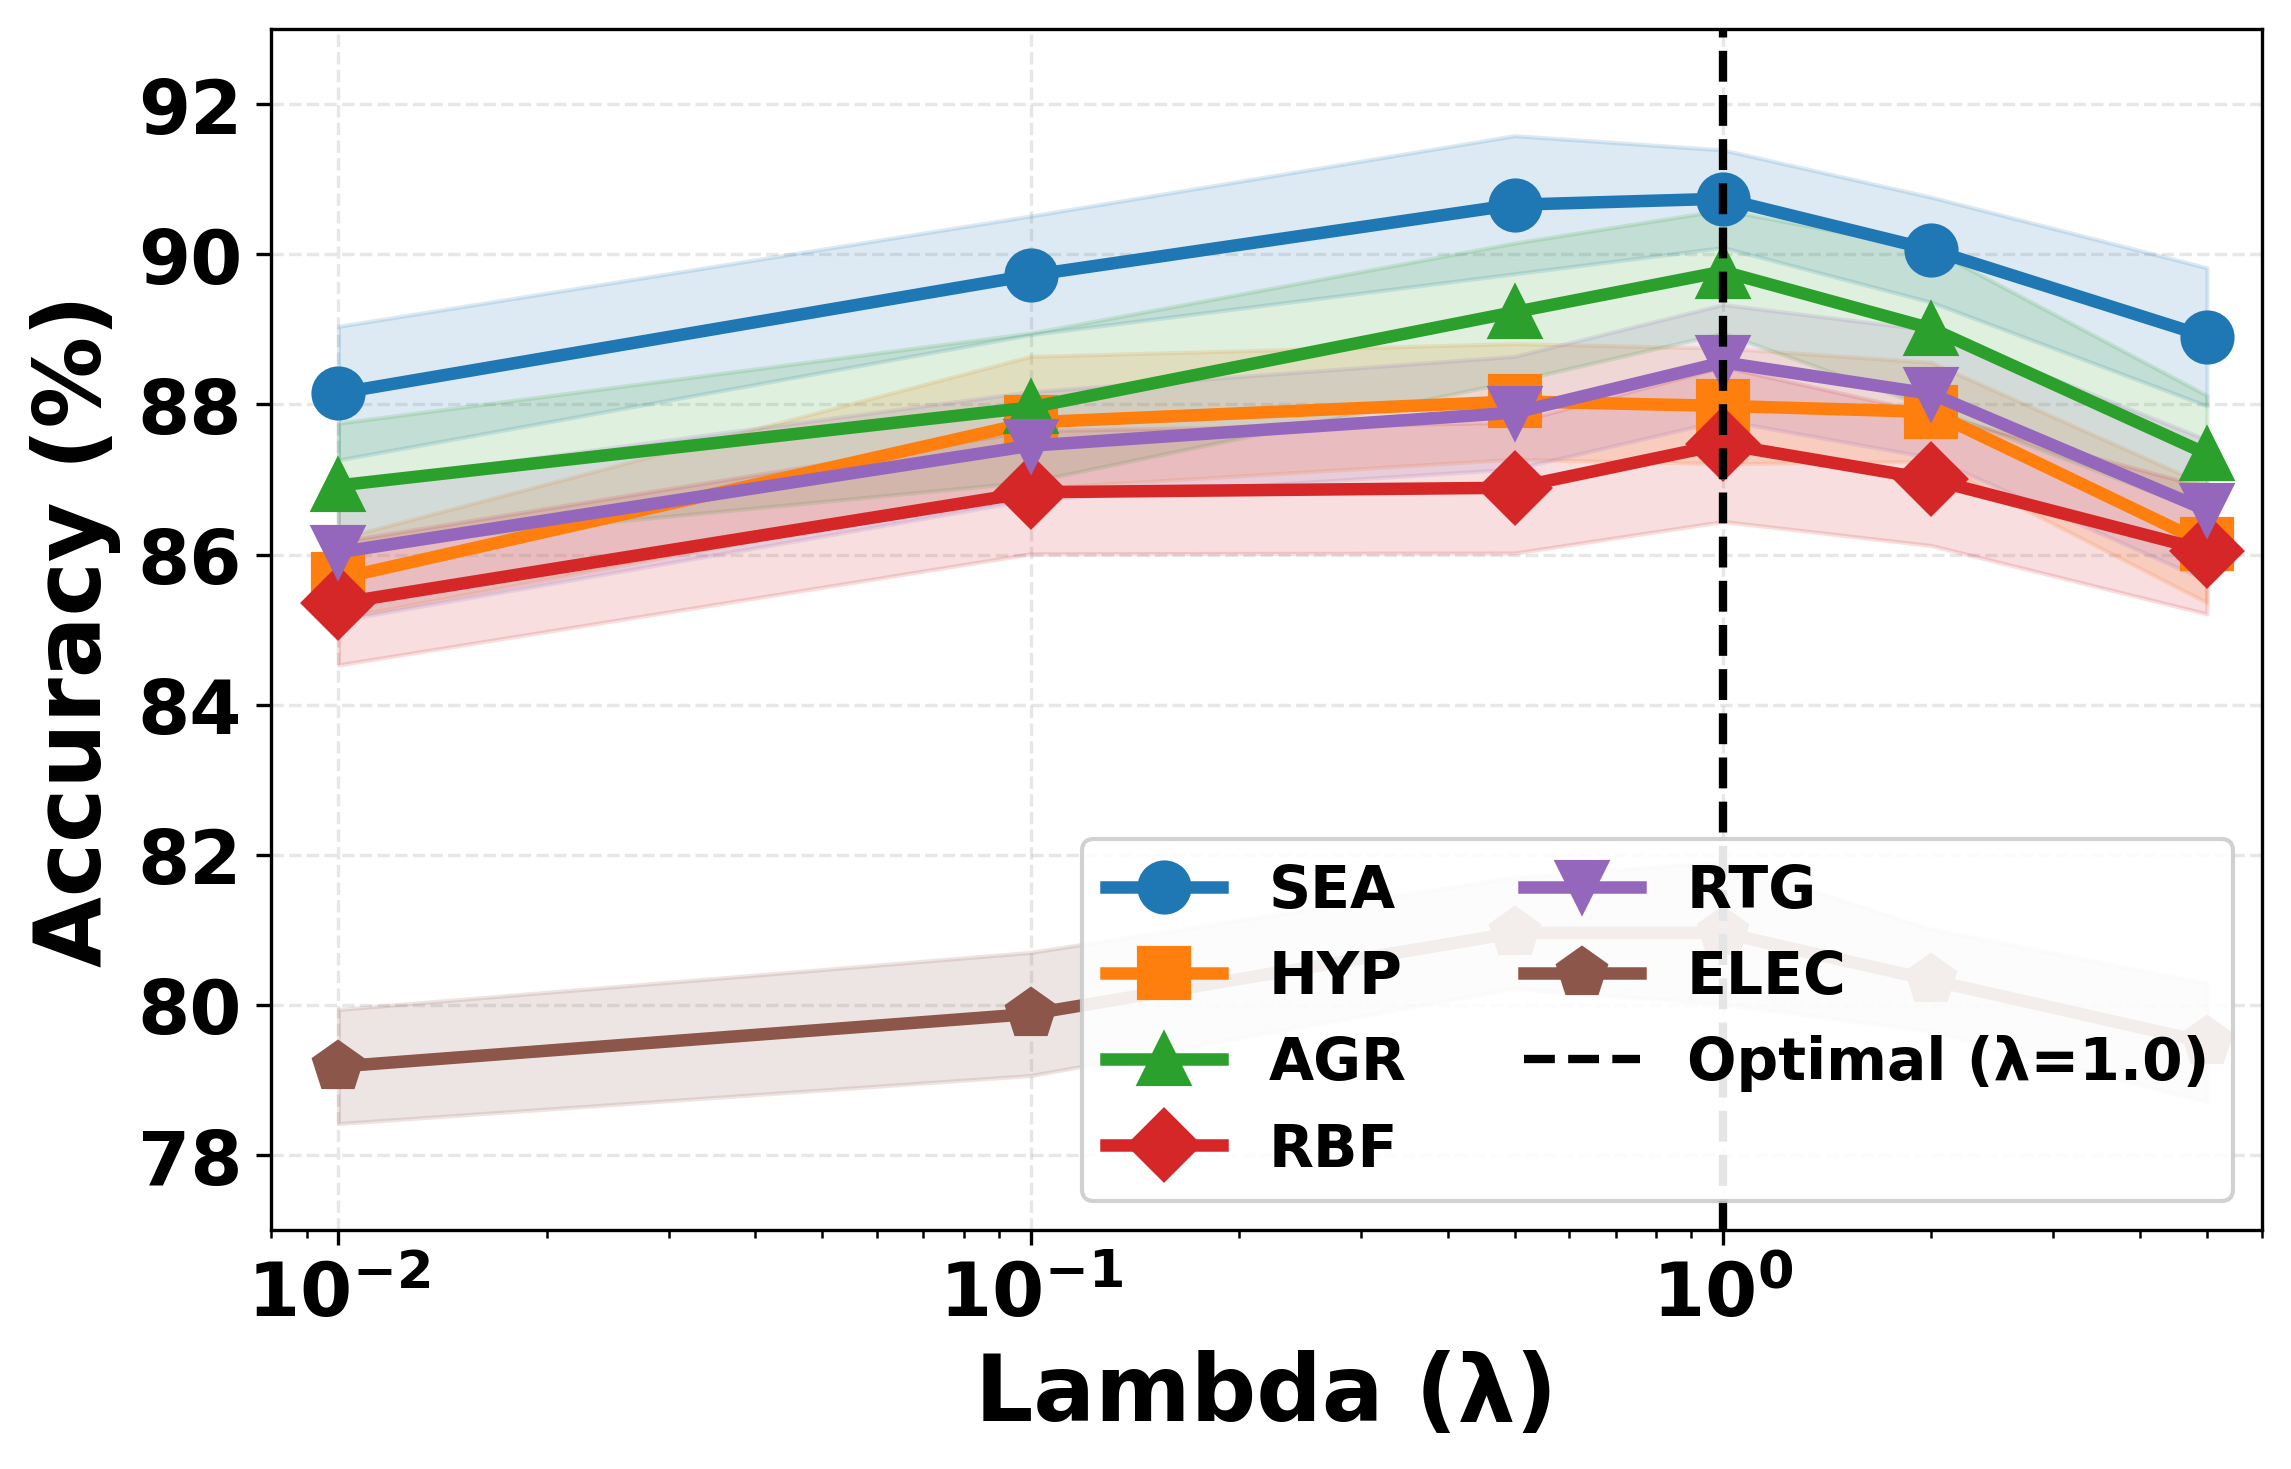
\includegraphics[width=\textwidth]{images/lambda_sensitivity.png}
        \caption{Regularization $\lambda$}
        \label{fig:lambda_sensitivity}
    \end{subfigure}
    \caption{Hyperparameter sensitivity analysis showing selection accuracy across different values of (a) window size, (b) exploration parameter, and (c) regularization parameter.}
    \label{fig:sensitivity}
\end{figure}

%\textbf{Computational Efficiency:} Figure~\ref{fig:time_memory} compares runtime and memory across methods. AutoDD processes instances at 0.29 ms per instance, which is 4.3 times faster than Meta-ADD at 1.25 ms per instance, while achieving higher accuracy. Memory usage is 7.5 MB for AutoDD, modest compared to Meta-ADD's 47.7 MB neural network overhead. Among the four state-of-the-art methods, AutoDD is faster than both PUDD at 0.33 ms and ADDM at 0.60 ms per instance. While MDDM is faster at 0.12 ms per instance, AutoDD achieves higher accuracy. %AutoDD occupies the favorable ``Fast + Low Memory'' quadrant alongside the classical detectors, while Meta-ADD falls in the ``Slow + High Memory'' region. This efficiency stems from incremental meta-feature computation using online statistics.

\textbf{Computational Efficiency:} For practical deployment in real-time streaming applications, computational efficiency is crucial. Figure~\ref{fig:time_memory} compares runtime and memory usage across all methods using GaussianNB as the base classifier. AutoDD achieves strong computational efficiency through its incremental meta-feature computation using online statistics, processing instances at 0.29 ms per instance. This is substantially faster than Meta-ADD at 1.25 ms per instance, making AutoDD 4.3 times more efficient while simultaneously achieving higher accuracy. Memory usage is 7.5 MB for AutoDD, which is modest compared to Meta-ADD's 47.7 MB neural network overhead. Among the state-of-the-art methods, AutoDD is faster than both PUDD at 0.33 ms and ADDM at 0.60 ms per instance. While classical detectors like MDDM are faster at 0.12 ms per instance, AutoDD delivers substantially higher accuracy with only modest additional overhead. This efficiency-accuracy trade-off makes AutoDD practical for deployment in high-velocity streaming scenarios where both performance and responsiveness are important.


% \begin{table}[!ht]
% \centering
% \caption{Computational efficiency}
% \label{tab:efficiency}
% \begin{tabular}{lcc}
% \toprule
% \textbf{Method} & \textbf{Time (ms/inst)} & \textbf{Memory (MB)} \\
% \midrule
% Page-Hinkley & 0.06 & 1.2 \\
% DDM & 0.08 & 1.9 \\
% EDDM & 0.10 & 2.2 \\
% MDDM & 0.12 & 5.4 \\
% ADWIN & 0.15 & 4.6 \\
% HDDM-A & 0.16 & 3.4 \\
% HDDM-W & 0.20 & 3.8 \\
% \textbf{AutoDD} & \textbf{0.29} & \textbf{7.5} \\
% PUDD & 0.33 & 5.3 \\
% KSWIN & 0.46 & 9.2 \\
% ADDM & 0.60 & 5.4 \\
% Meta-ADD & 1.25 & 47.7 \\
% \bottomrule
% \end{tabular}
% \end{table}


\begin{figure}[!ht]
    \centering
    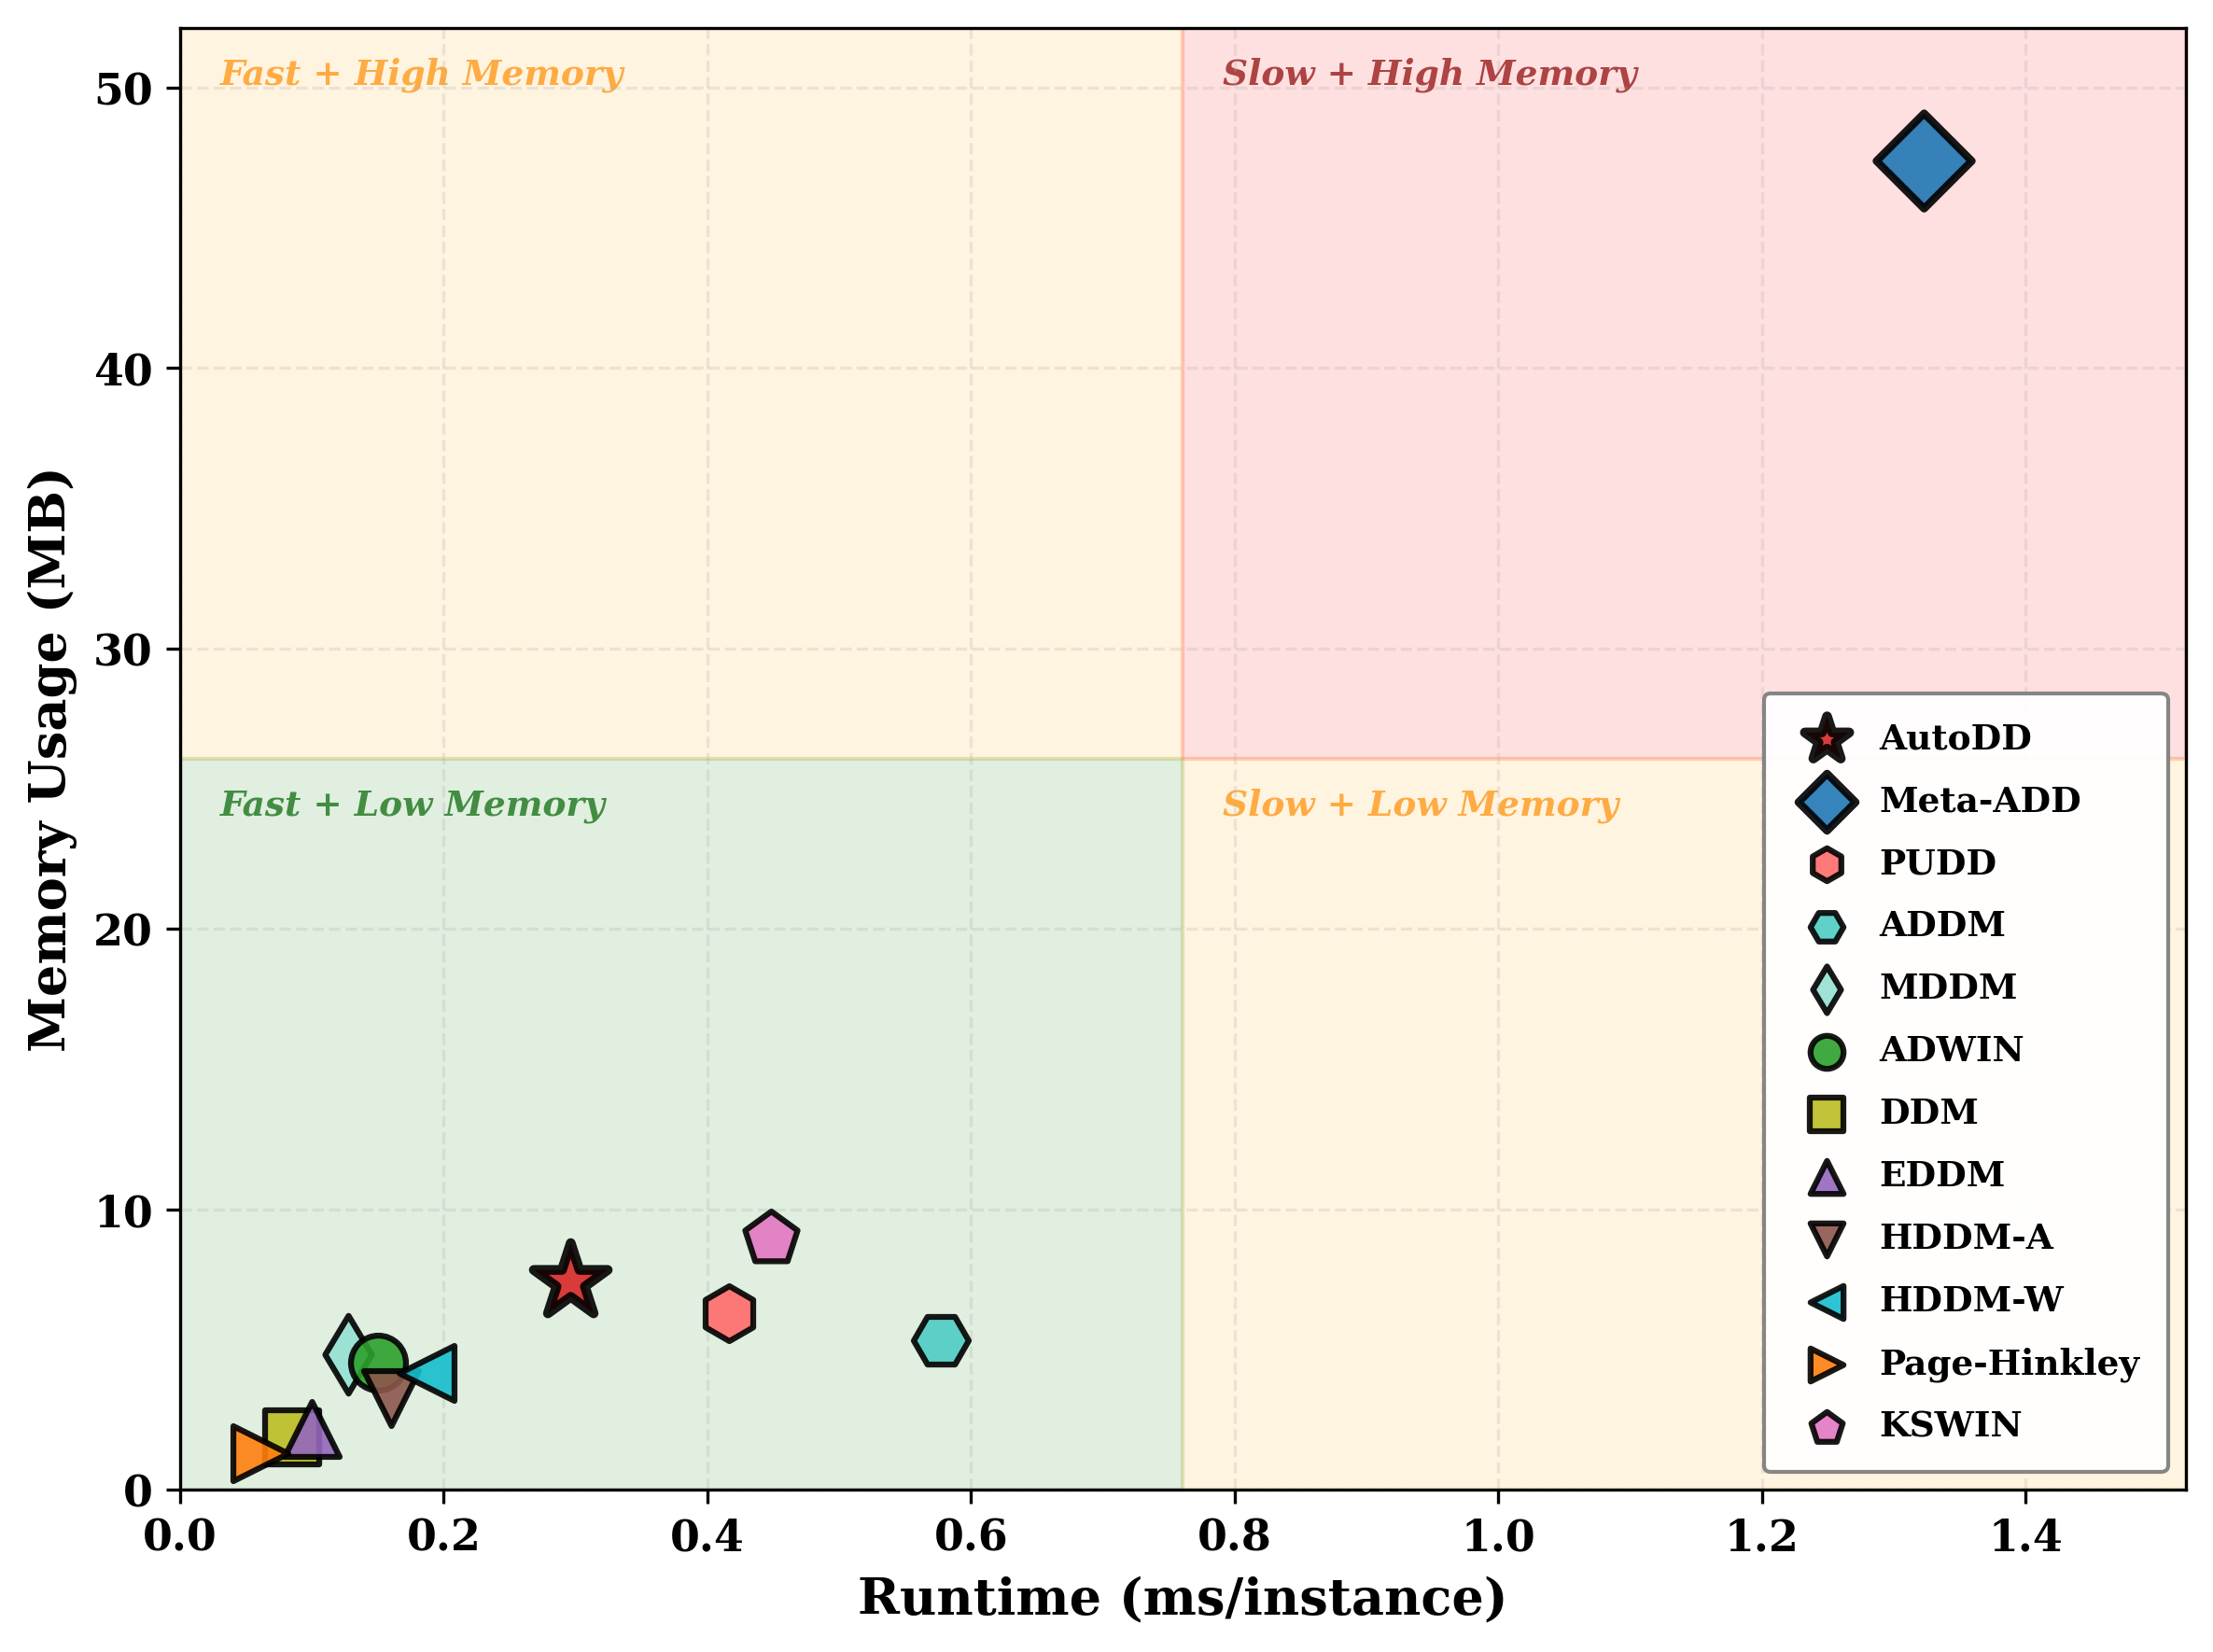
\includegraphics[width=0.75\columnwidth]{images/time_memory_gaussiannb.png}
    \caption{Runtime vs. memory trade-off.}
    \label{fig:time_memory}
\end{figure}

% \section{Discussion}
% \label{sec:discussion}

% A key design choice in AutoDD is the use of accuracy drop as a proxy for evaluating drift detection quality. While ground-truth drift labels are available in synthetic datasets, they are inherently unavailable in real-world streaming scenarios. Our reward function measures the downstream impact of detection decisions by rewarding detections that coincide with performance degradation while penalizing false alarms and missed drifts. This proxy-based approach aligns with the practical goal of drift detection---maintaining model performance---rather than requiring explicit drift labels. To ensure fair comparison, we use complete model reset consistently across AutoDD and all baselines, ensuring that observed performance differences reflect detector selection quality rather than adaptation strategy effects.

% AutoDD's portfolio comprises seven classical drift detectors spanning statistical, error-based, and distribution-based paradigms. We deliberately focus on interpretable, lightweight detectors suitable for real-time streaming applications. AutoDD introduces modest overhead (0.29 ms/instance) due to meta-feature extraction and LinUCB updates, justified by 4--8\% accuracy improvements over fixed detectors while remaining 4.3$\times$ faster than Meta-ADD. The incremental computation of online statistics ensures scalability to high-velocity streams. We acknowledge several limitations: AutoDD's performance on gradual drift is slightly lower than Meta-ADD on certain datasets, suggesting that learned drift-type representations may complement our meta-feature approach. The window size $w=100$ represents a trade-off between detection responsiveness and statistical stability. Some meta-features require careful implementation, including histogram-based KL divergence with adaptive binning and approximate $k$-NN with $k=5$. Finally, AutoDD assumes immediate label availability; under substantial delays, unsupervised proxy rewards could enable label-efficient operation.

\section{Conclusion}
\label{sec:conclusion}

We propose AutoDD, a novel framework that automatically selects and configures drift detectors for data streams. The framework extracts comprehensive meta-features and employs a two-level hierarchical selection strategy using LinUCB for detector selection and Thompson Sampling for hyperparameter configuration. Theoretical analysis provides sublinear regret bounds guaranteeing convergence to optimal detector-configuration pairs. Extensive experimental results on synthetic and real-world datasets demonstrate that AutoDD achieves significant improvements over fixed detector baselines and state-of-the-art methods while requiring no expert intervention. Future work includes incorporating multi-objective optimization to balance accuracy, detection latency, and computational efficiency. We also plan to expand AutoDD to different types of data stream problems, including unsupervised drift detection scenarios where labels are unavailable. Additionally, exploring better adaptation strategies beyond model reset, such as incremental learning and ensemble updating, represents a promising direction for further improving post-drift recovery.


\bibliographystyle{named}
\bibliography{references}

\end{document}